\chapter{The growth of social groups}

\section{Social groups}


Two popular online platforms \textbf{Reddit} and \textbf{Meetup} are organized into different groups. On Reddit \footnote{https://www.reddit.com/}, users create subreddits, where they share web content and discussion on specific topics, so their interactions are online through posts and comments. The Meetup groups \footnote{www.meetup.com}, are also topic-focused, but the primary purpose of these groups is to help users in organizing offline meetings. As meetings happen face-to-face, Meetup groups are geographically localized, so we'll focus on groups created in two towns, London and New York. 

The Meetup data cover groups created from $2003$, when the Meetup site was founded, until $2018$, when using the Meetup API we downloaded data. We extracted the groups from London and New York that were active for at least two months. There were 4673 groups with 831685 members in London and $4752$ groups with 1059632 members in New York. For each group, we got information about organized meetings and users who attended them. From there, for each user, we can find the date when the user participated in a group event for the first time; it is considered the date when the user joined a group. 

The Reddit data were downloaded from https://pushshift.io/ site. This site collects posts and comments daily; data are publicly available in JSON files for each month. The selected subreddits were created between 2006 and 2011, we also filtered those active in 2017. We removed subreddits active for less than two months. The obtained dataset has 17073 subreddits with $2 195 677$ active members. For each post, we extracted the subreddit-id, user-id and the date when the user created the post. Finally, we selected the date when each user posted on each subreddit for the first time.

\subsection{The empirical analysis of social groups}

Both datasets have the same structure $(group-id, user-id, timestamp)$, where the timestamp was the date when the user joined the group. For each time step, we can calculate the number of new members in each group $N_i(t)$, and the group size $S_{i}(t)$. The group size at time step $t$ is $S_{i}(t)=\sum^{k=t}_{k=t_{0}}N_{i}(t)$, where $t_0$ is month when group is created. The group size is increasing in time, as we do not have information if the user left the group. Also we calculate the growth rate, as the logarithm of successive sizes $R = log(S_{i}(t)/S_{i}(t-1))$. 

Even though Meetup and Reddit are different online platforms, we find some common properties of these systems; see figure \ref{fig:data1}. The number of groups and the number of new users grow exponentially. Still, subreddits are larger groups than Meetups. The distribution of groups sizes follows the log-normal distribution:
\begin{equation}
P(S)=\frac{1}{S\sigma\sqrt{2\pi}}exp(-\frac{(\ln(S)-\mu)^{2}}{2\sigma^{2}})
\label{eq:log}
\end{equation}
where $S$ is the group size and $\mu$, and $\sigma$ are parameters of the distribution.
The group sizes distribution of Subreddits is a broad log-normal distribution that resembles the power law. Still, we used the loglikelihood ratio method and showed that log-normal distribution is better than the power-law. More details are given in the result section. 


%We used package \cite{powerlaw} to fit Eq. \ref{eq:log} to Reddit and Meetup data and found that distribution of groups sizes for Meetup groups in London and New York follow similar distributions with the values of parameters $\mu= -0.93$, $\sigma = 1.38$ and $\mu=-0.99$ and $\sigma=1.49$ for London and New York respectively. The distribution of sizes of subreddits also has the log-normal shape with parameters $\mu= -5.41$ and $\sigma = 3.07$. Even though these distributions are from the same class, for subreddits we find broader distribution that may resemble power-law distribution. Our analysis shown in Supportive Information (SI) confirms that the distribution exhibits a log-normal behavior, see SI-Table 1 and SI-Fig. 1. 

\begin{figure}[h]
	\centering
	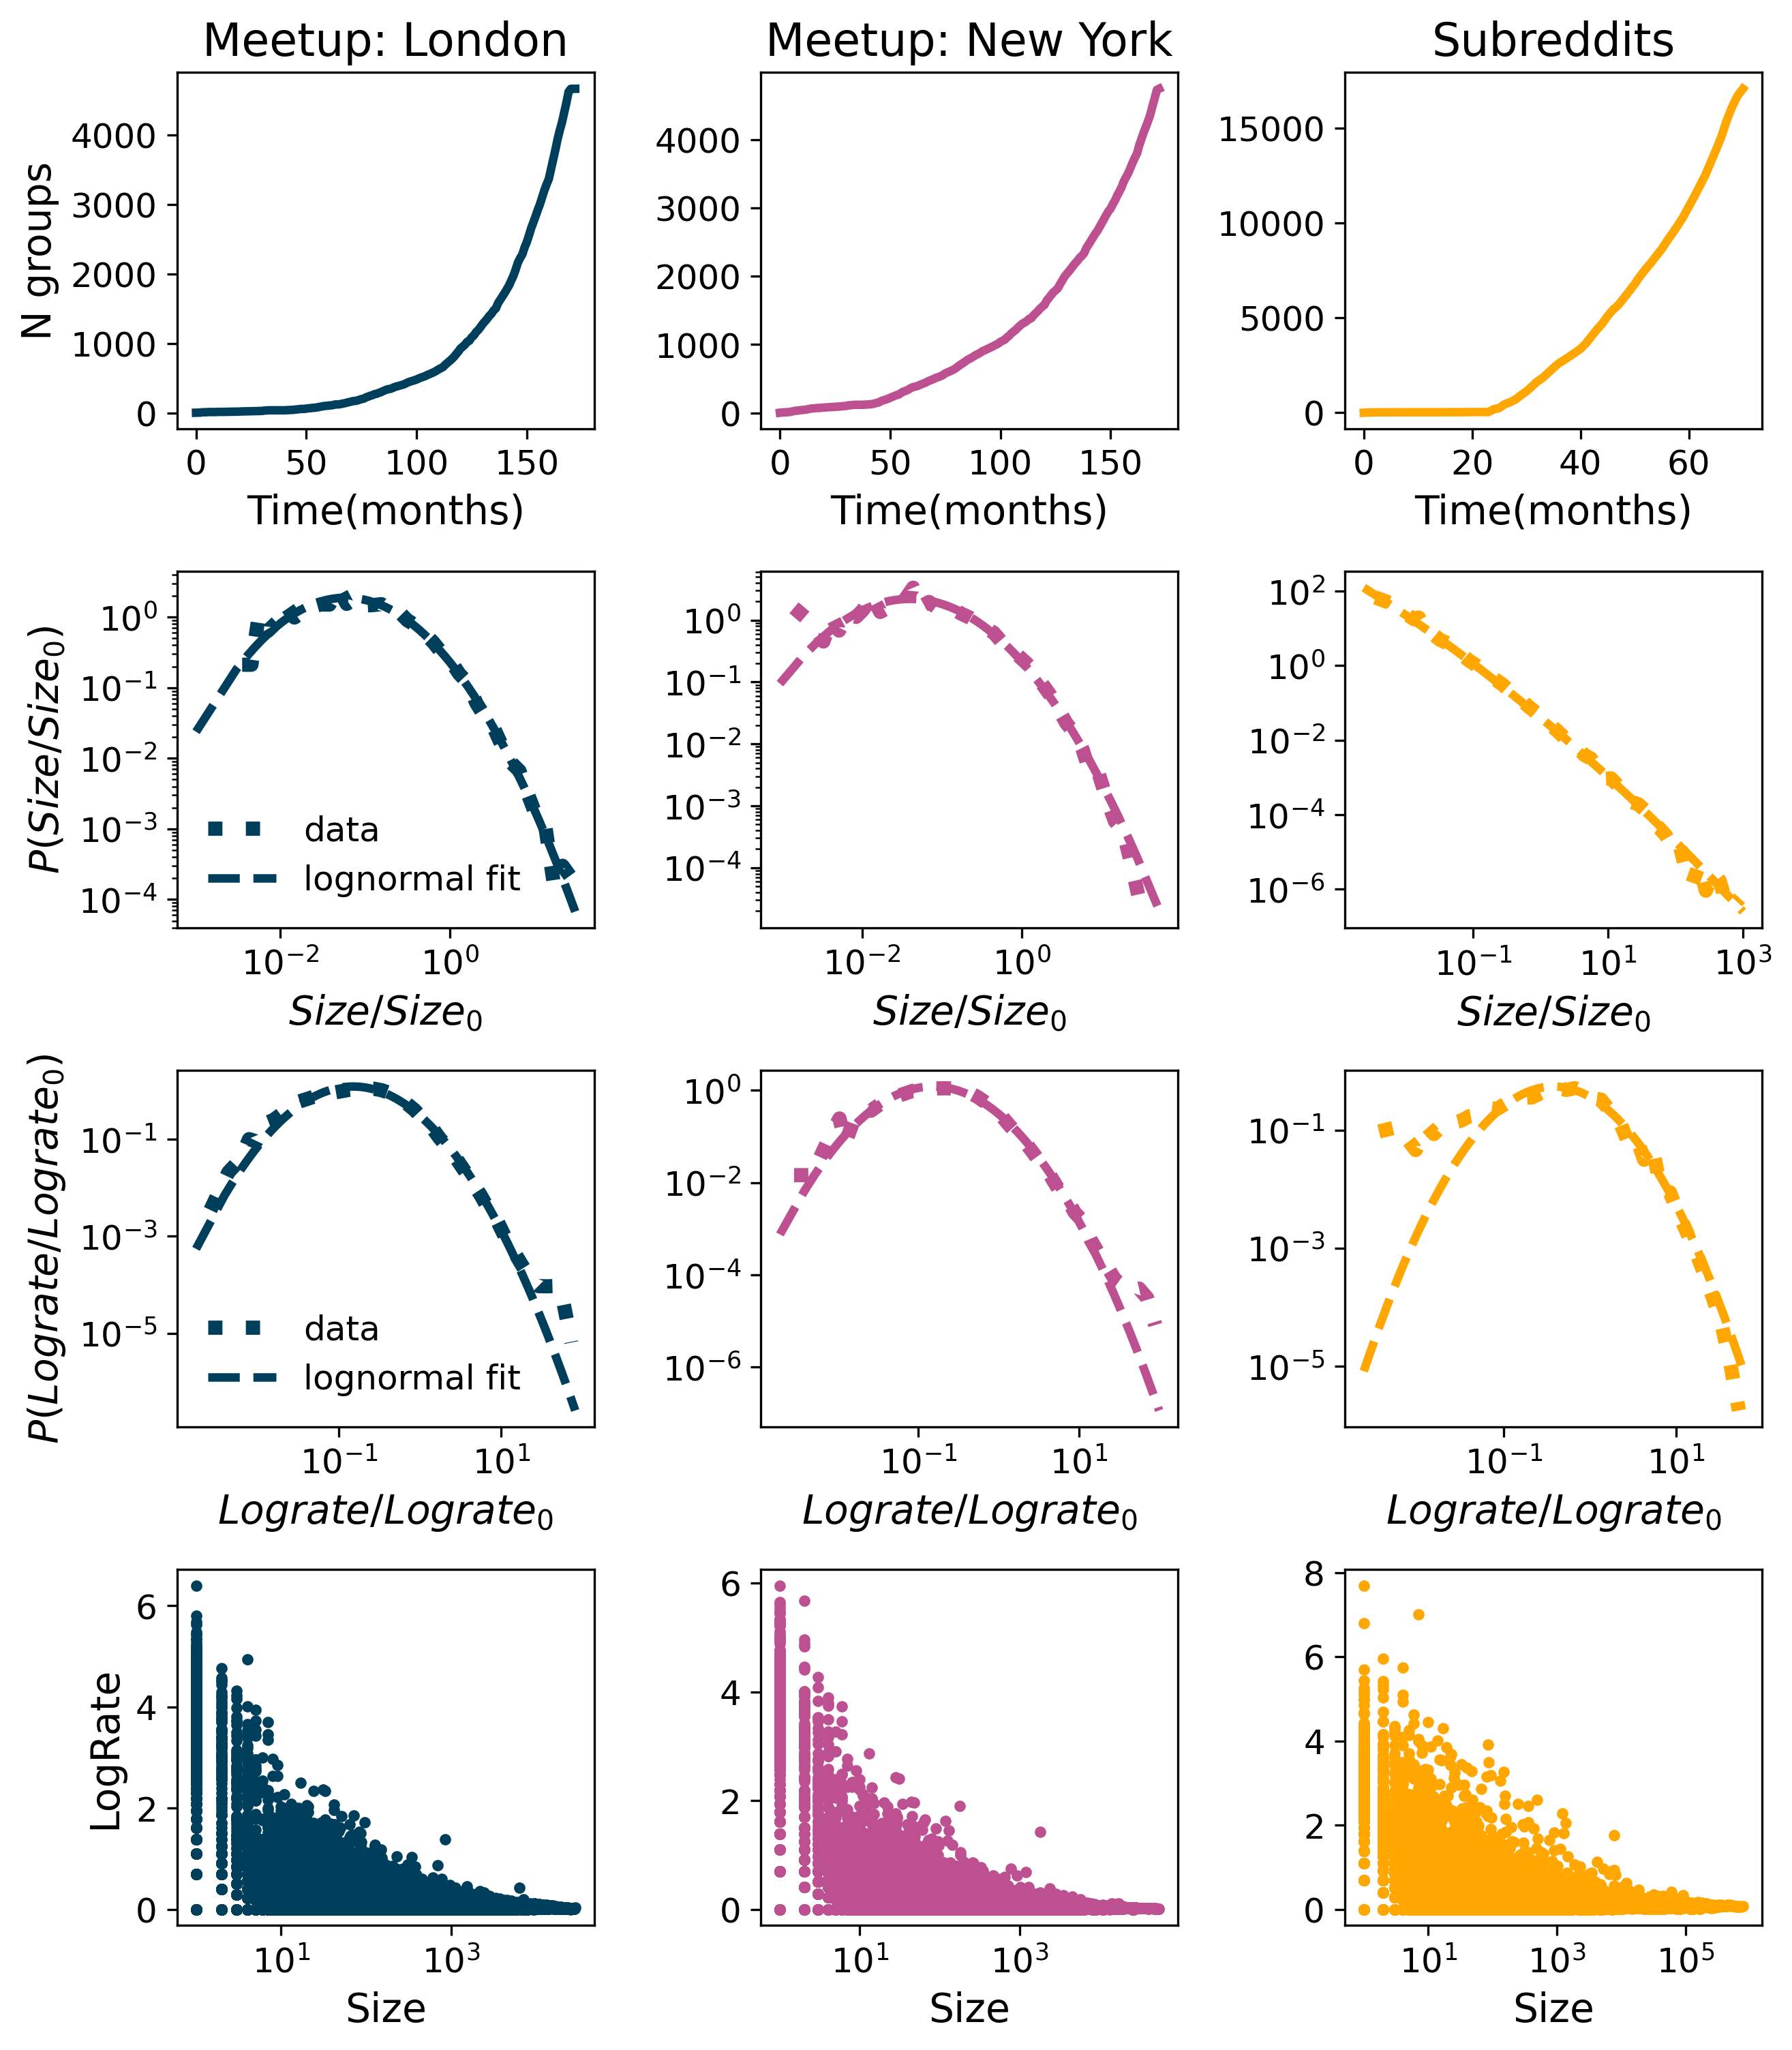
\includegraphics[width=0.8\linewidth]{Figures/figures/Fig2.png}
	\caption{The number of groups over time, normalized sizes distribution, normalized log-rates distribution and dependence of log-rates and group sizes for Meetup groups created in London from 08-2002 until 07-2017 that were active in 2017 and subreddits created in the period from 01-2006 to the  12-2011 that were active in 2017. }
	\label{fig:data1}
\end{figure}  

The multiplicative process \cite{mitzenmacher2004brief} is the simplest way to generate the lognormal distribution. It is also known as Gibrat law and it states that the growth rates are uncorrelated $R = log\frac{S_t}{S_{t-\Delta t}}$. The distribution of sizes $P(S)$ follow lognormal while the distribution of log rates should follow the normal distribution or, as shown in many studies explained with Laplacian (“tent shaped“) distribution \cite{mondani2014fat}, \cite{fu2005growth}. For Meetup and Reddit, we find that the lognormal distribution fits logrates. Furthermore, logrates depend on the group size. For these reasons, the growth of social groups can not be explained with Gibrat law, \cite{frasco2014spatially, qian2014origin}.

If we aggregate the groups created in the same year $y$, and each group size normalize with average size $<S^y>$, $s^{y}_{i}=S^{y}_{i}/<S^{y}>$ we will find that group sizes distributions for the same dataset and different years fall on the same line, figure \ref{fig:scale}. The growth of the social groups has universal behavior. It is independent on the size of the group, that is showed by rescaling dataset. Also, the growth is universal in time, and the group sizes distribution do not change from year to year. Same characteristics are observed for the distribution of normalized logrates, see figure \ref{fig:scale}. 



%The number of groups and users grows exponentially. Group size distribution follow lognormal distribution but Gibrat-law is not applicable as logrates distribution deviates from normal distribution. Indications of the universal scaling in these datasets and the common properties of the 





%While the forms of communication between members and activities that members engage in differ in those two systems, some common properties exist between them. Members can form a new groups and join existing ones in both systems. Furthermore, each member can belong to an unlimited number of groups. For these reasons, we can use the same methods to study and compare the formation of groups in Reddit and Meetup. 


%While these two systems differ in means of communication between their members and activities their members engage in, there are certain common properties that enable us to use same methods to study the growth of groups in these systems and make a comparative analysis of this growth. In both systems, members can create new groups and join existing ones. One member can belong to unlimited number of groups/subreddits at the same time. The number of groups in the systems is also unlimited. For each meetup group we have an information on when member has attended first group event. Based on this information we can infere the size of each group for each month. For a subreddit we have a detailed information about members' activity and thus we have an information when a user made a first post in specific subreddit. This moment is considered as the moment when the member has joined the subreddit and became an active member. In our case we do not take into account when a member leaves a group or subreddit, since this kind of information is not available to us. For these reasons, the size of considered groups is non-decreasing function. 


\begin{figure}[h]
	\centering
	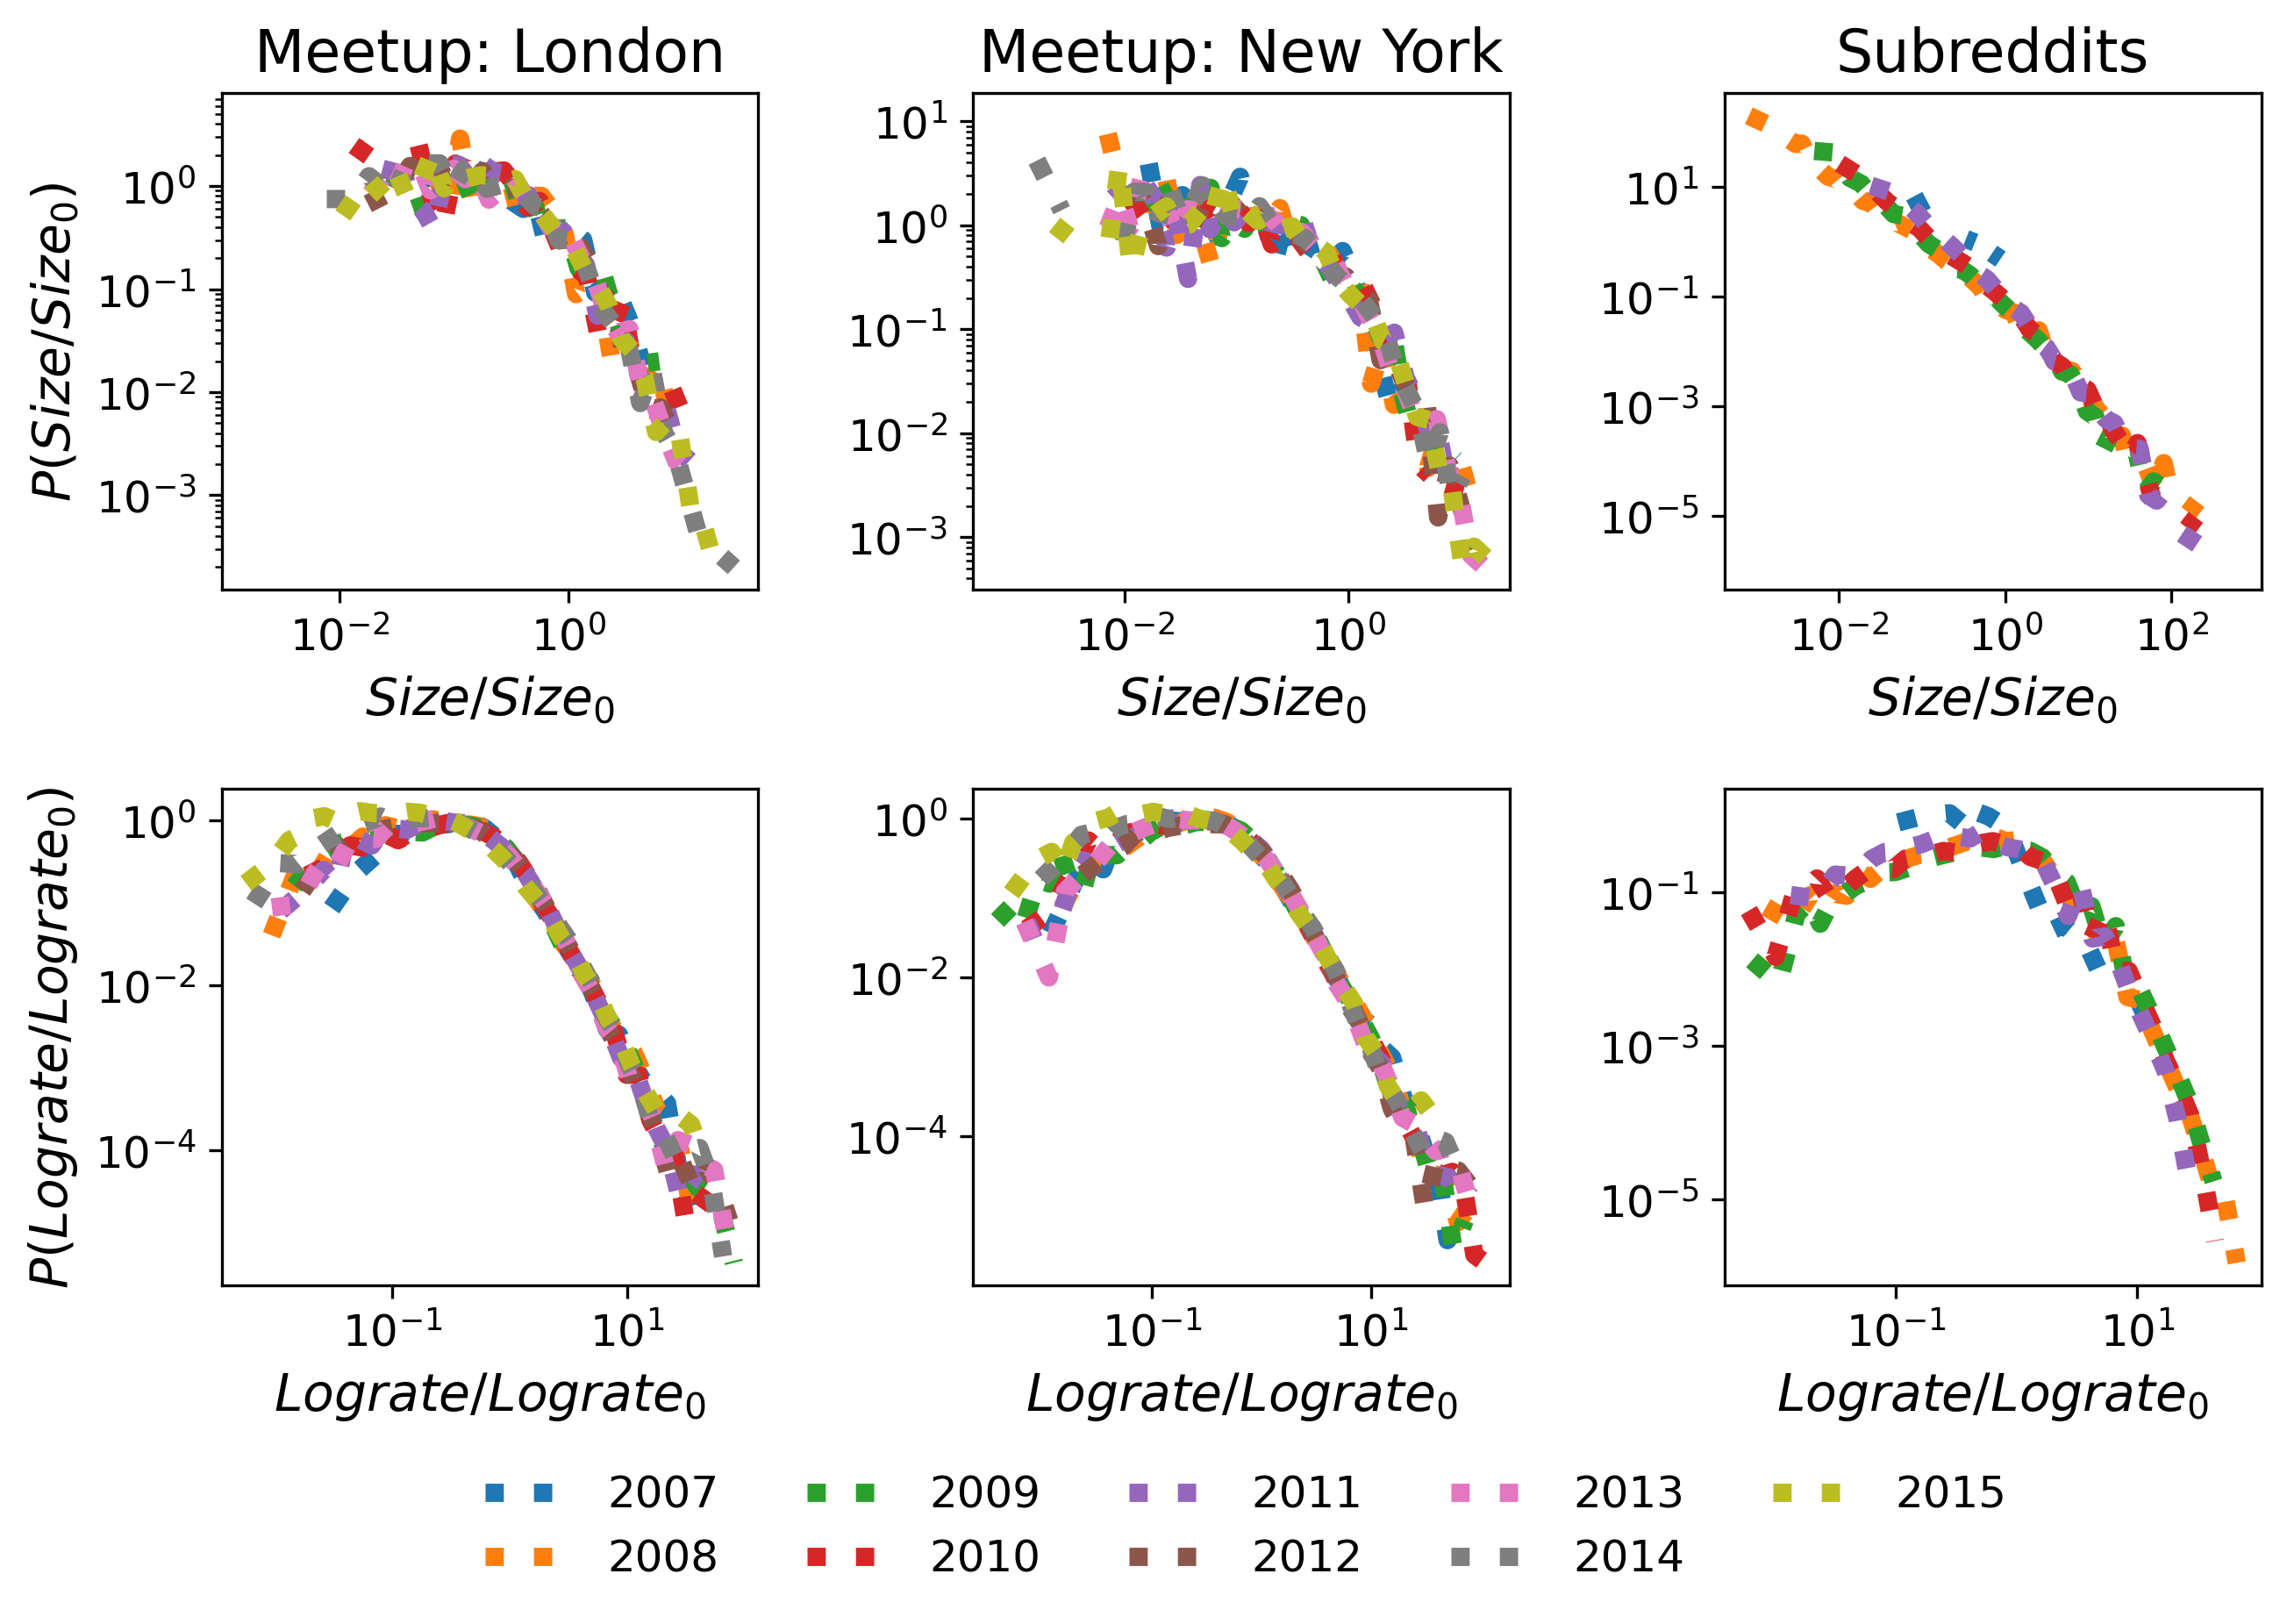
\includegraphics[width=0.8\linewidth]{Figures/figures/Fig1.png}
	\caption{The figure shows the groups' sizes distributions and log-rates distributions. Each distribution collects groups founded in the same year and is normalized with its mean value. The group sizes are at the end of 2017 for meetups and 2011 for subreddits. }
	\label{fig:scale}
\end{figure}


\section{The groups growth model}


\begin{figure}[H]
	\centering
	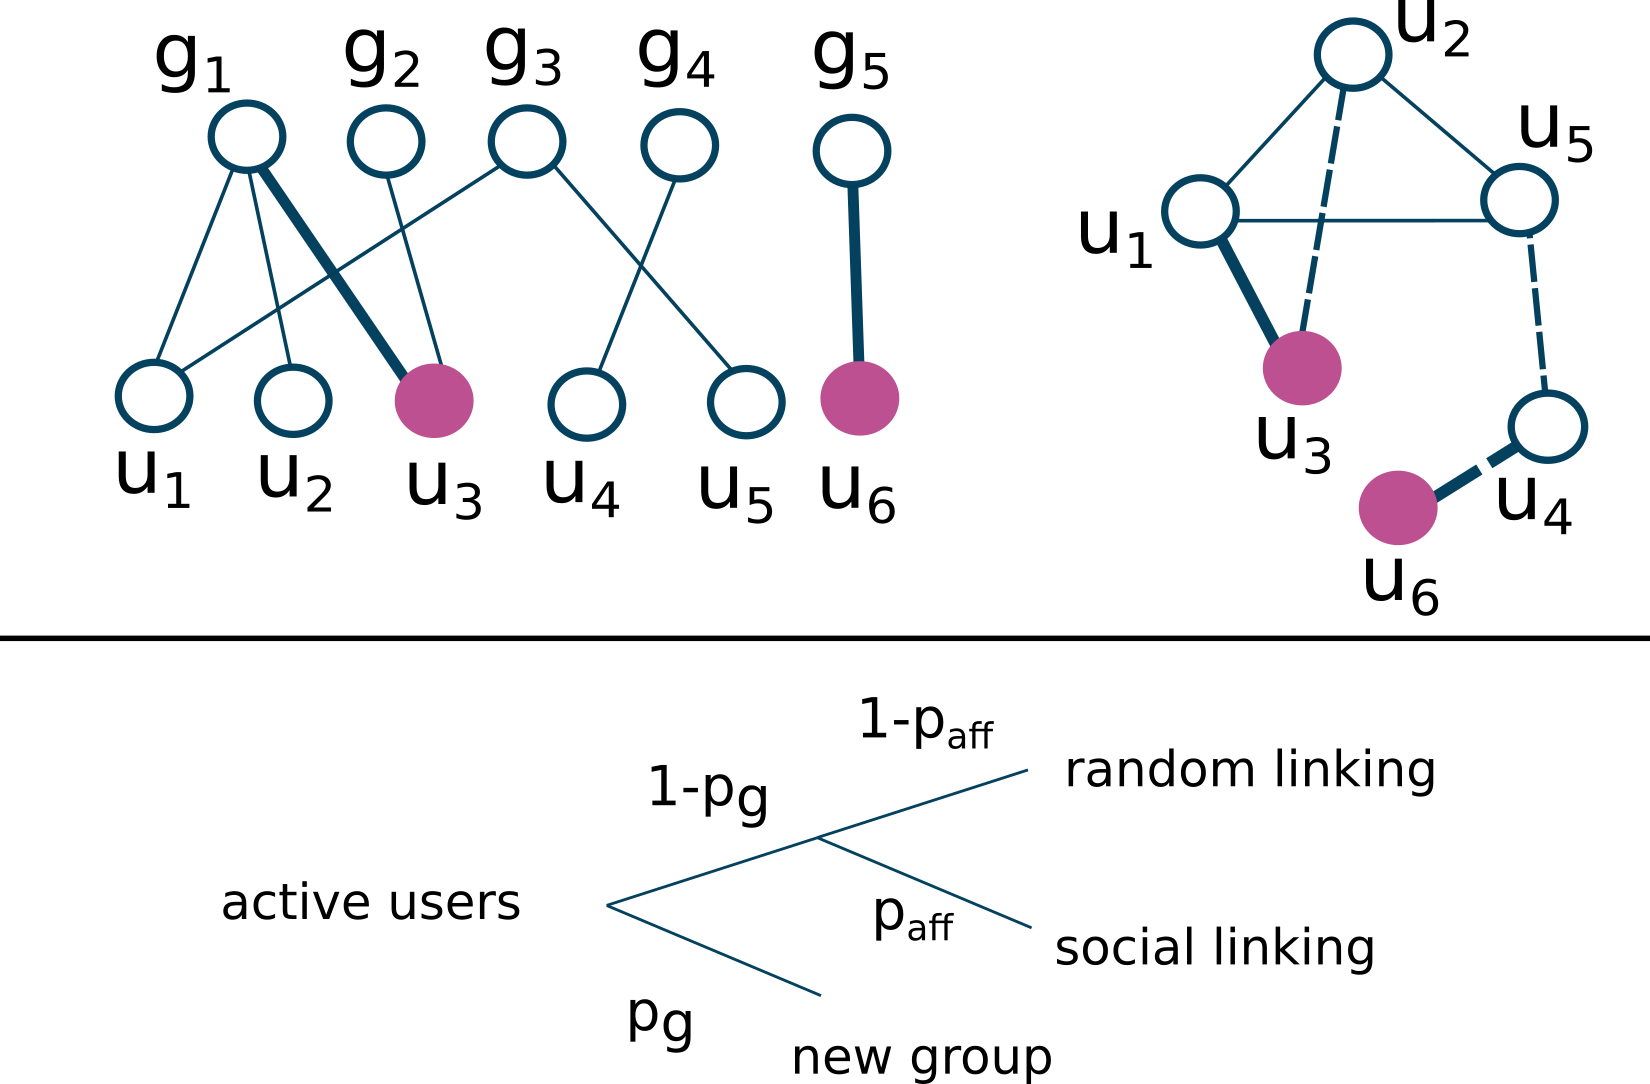
\includegraphics[scale=0.5]{Figures/figures/test.png}
	\caption{The top panel shows bipartite (member-group) and social (member-member) network. Filled nodes are active members, while thick lines are new links in this time step. In the social network dashed lines show that members are friends but still do not share same groups. The lower panel shows model schema. \textbf{Example:} member $u_6$ is a new member. First it will make random link  with node $u_4$, and then with probability $p_g$ makes new group $g_5$. With probability $p_a$ member $u_3$ is active, while others stay inactive for this time step. Member $u_3$ will with probability $1-p_g$ choose to join one of old groups and with probability $p_{aff}$ linking is chosen to be social. As its friend $u_2$ is member of group $g_1$, member $u_3$ will also join group $g_1$. Joining group $g_1$, member $u_3$ will make more social connections, in this case it is member $u_1$.}
	\label{fig:schema}
\end{figure}

\begin{figure}[H]
	\centering
	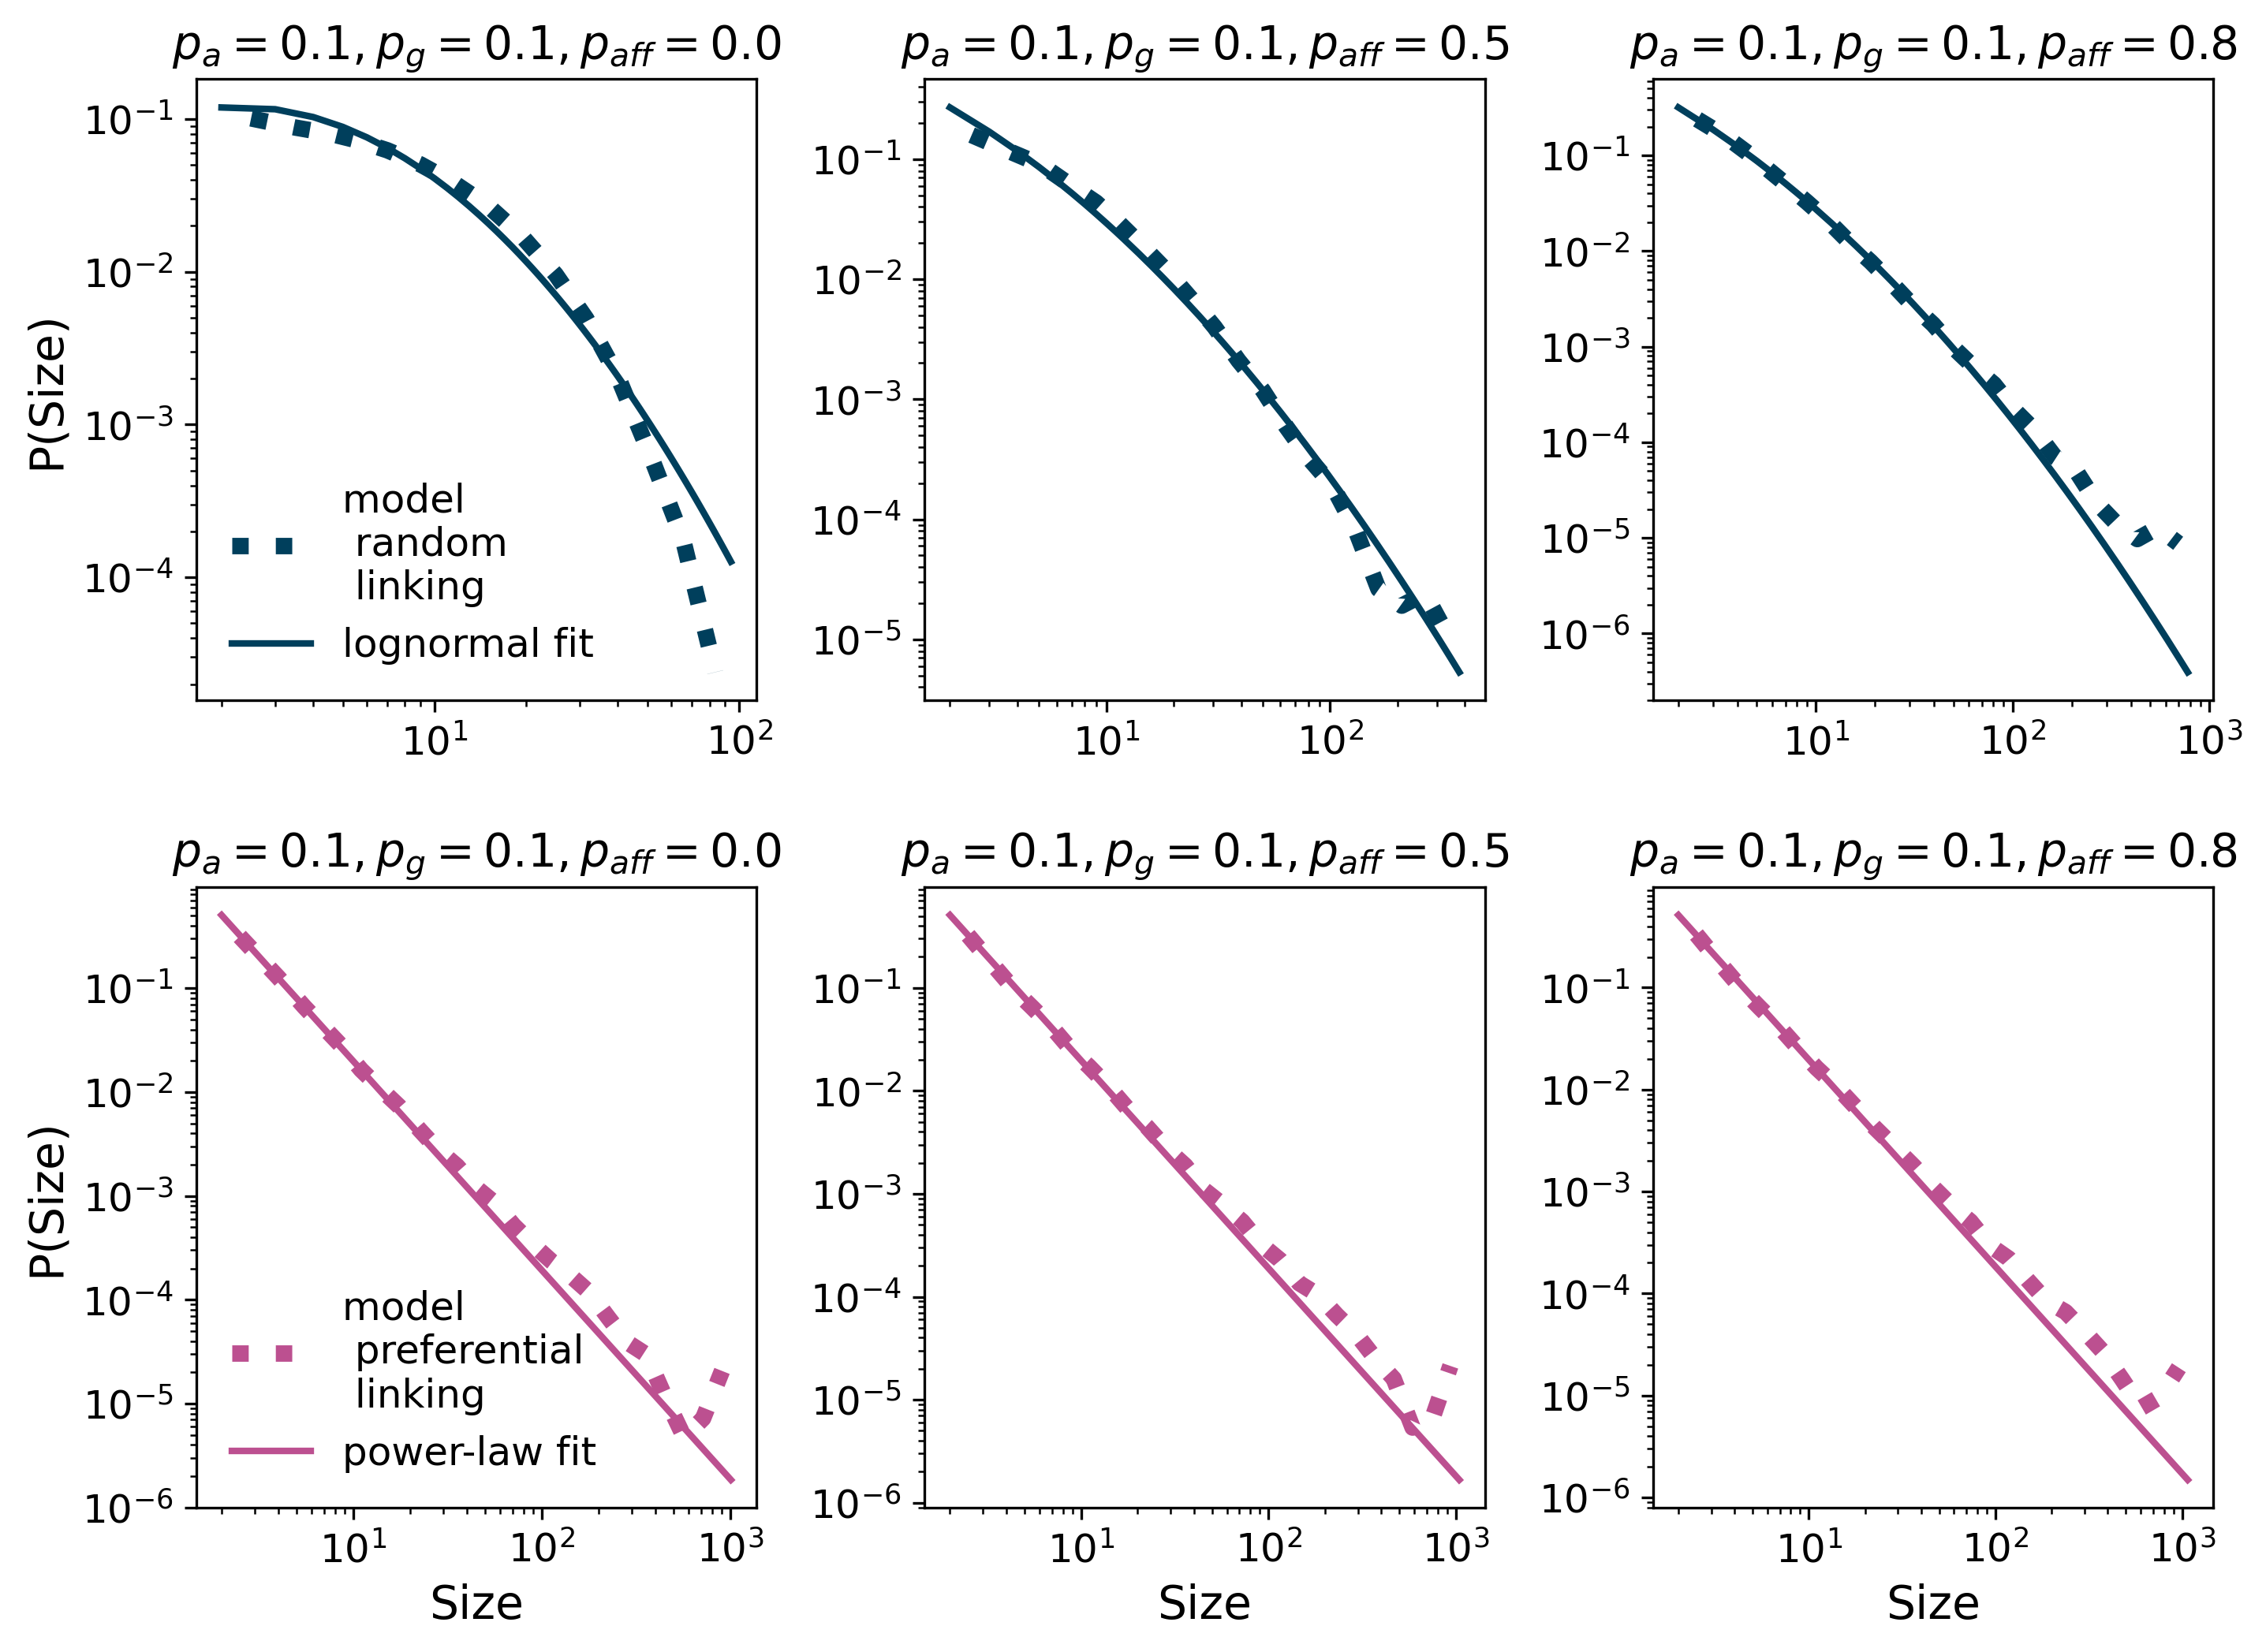
\includegraphics[width=0.8\linewidth]{figures/model_N30.png}
	\caption{Groups sizes distributions for groups model, where at each time step the constant number of users arrive, $N=30$ and old users are active with probability $p_a=0.1$. Active users make new groups with probability $p_g=0.1$, while we vary affiliation parameter $p_{aff}$. With probability, $1-p_{aff}$, users choose a group randomly. The group sizes distribution (top row) is described with a log-normal distribution. With higher affiliation parameter, $p_{aff}$, distribution has larger width. The bottom row presents the case where with probability $1-p_{aff}$ users have a preference toward larger groups. For all values of parameter $p_{aff}$, we find the power-law group sizes distribution.}
	\label{fig:model_comp}
\end{figure}


\clearpage
\newpage
\section{Results}
\begin{figure}[H]
	\centering
	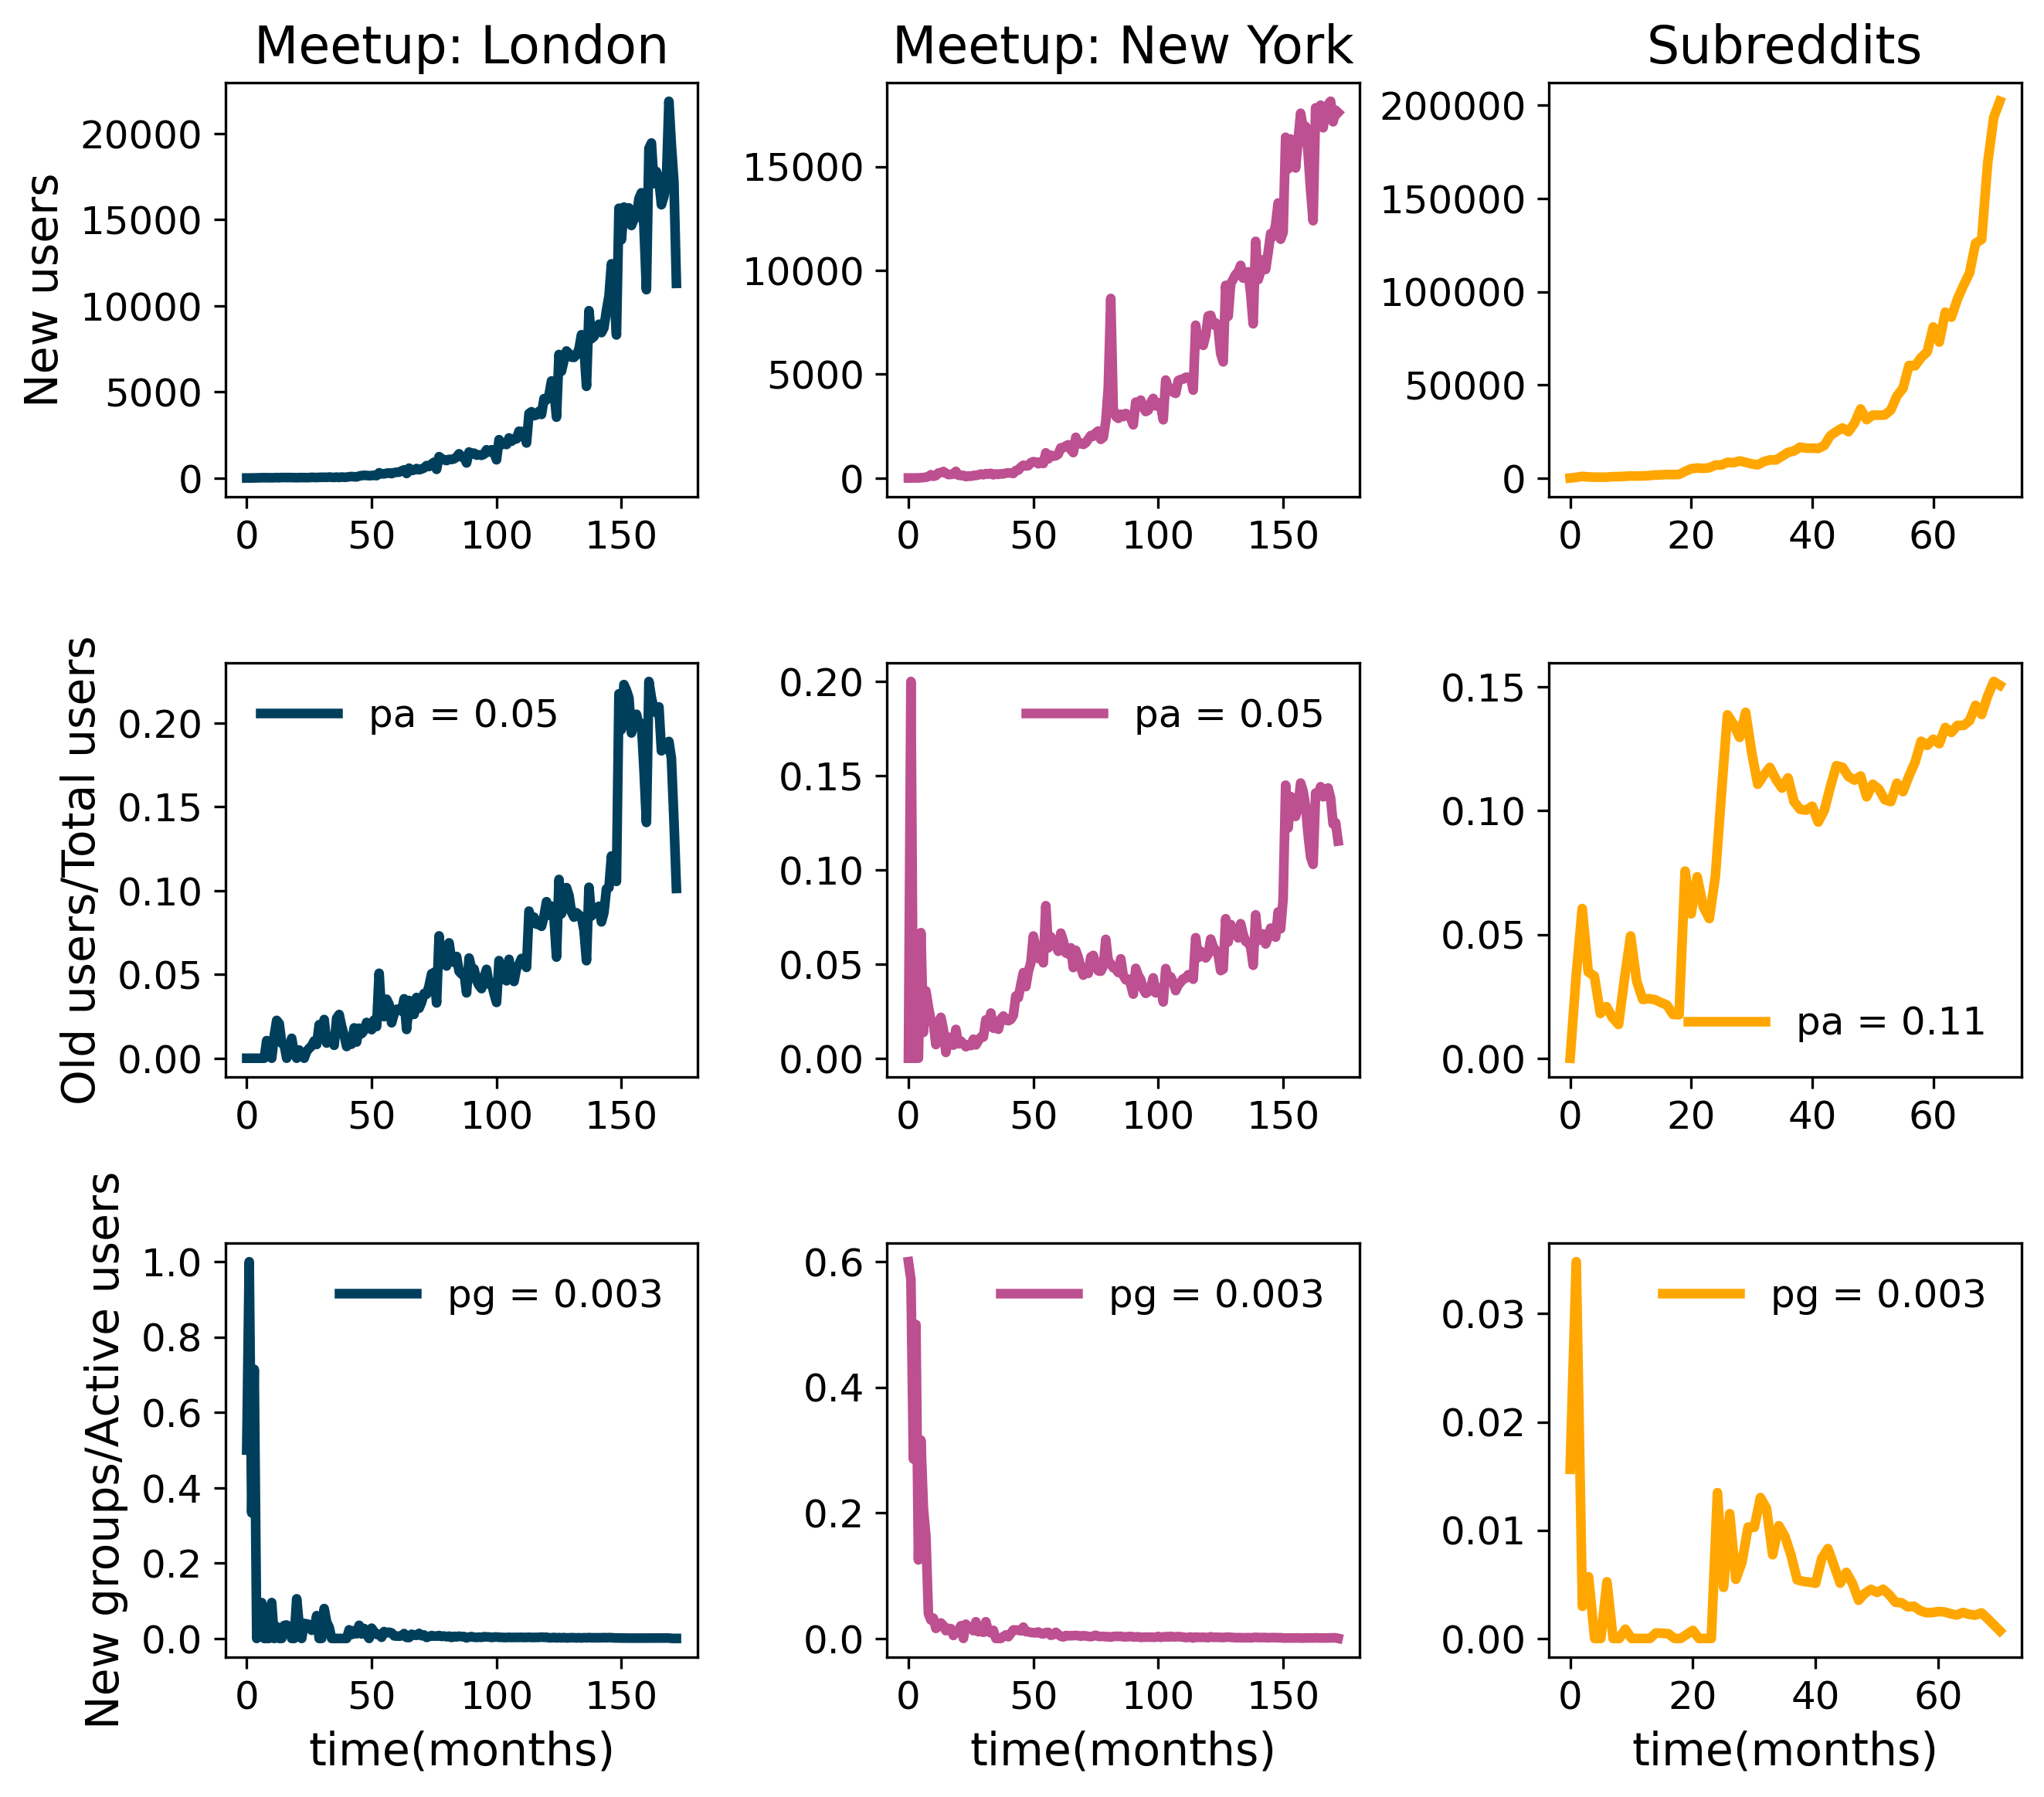
\includegraphics[width=0.8\linewidth]{Figures/figures/Fig3.png}
	\caption{The time series of number of new members (top panel), ratio between old members and total members in the system (middle panel), and ratio between new groups and active members(bottom panel) for Meetup groups in London,  Meetup groups in New York, and subreddits. }
	\label{fig:fig5}
\end{figure}






%Social groups, informal or formal, are mesoscopic building elements of every socio-economic system that direct its emergence, evolution, and disappearance \cite{}. The examples span from countries, economies and science to society in general. Settlements, villages, towns and cities are formal and highly structured social groups of countries. Their organisation and growth determine the functioning and sustainability of every society \cite{barthelemy2016structure}. Companies are the building blocks of an economic system and their dynamics are important indicators of the level of its development \cite{hidalgo2009building}. Scientific conferences, as scientific groups, enable fast dissemination of the latest results, exchange and evaluation of ideas as well as a knowledge extension, and thus are an integral part of science \cite{smiljanic2016theoretical}. The membership of individuals in various social groups, online and offline, can be essential when it comes to the quality of their life \cite{montazeri2001anxiety, davison2000talks, cho2012tea}. Therefore, it is not surprising that the social group emergence and evolution are at the center of the attention of many researchers \cite{aral2012identifying,gonzalez2013broadcasters, torok2013opinions, yasseri2012dynamics}.

 
%Along with massive data sets comes the need to develop methods and tools for their analysis and modeling. Methods and paradigms from statistical physics have proven to be very useful in studying the structure and dynamics of social systems \cite{castellano2009statistical}. The main argument for using statistical physics to study social systems is that they consist of many interacting individuals. Due to this, they exhibit different patterns in their structure and dynamics, commonly known as \textit{collective behavior}. While building units of a social systems can be characterized by many different properties, only few of them enforce collective behavior in the systems. The phenomenon is known as \textit{universality} in physics and is commonly observed in social systems such as in voting behavior \cite{chatterjee2013universality}, or scientific citations \cite{radicchi2008universality}. It indicates the existence of the universal mechanisms that govern the dynamics of the system \cite{}.


%The availability of large-scale and long-term data on various online social groups has enabled the detailed empirical study of their dynamics. The focus was mainly on the individual groups and how structural features of social interaction influence whether individuals will join the group \cite{backstrom2006group} and remain its active members \cite{smiljanic2016theoretical, smiljanic2017associative}. The study on LiveJournal \cite{backstrom2006group} groups has shown that decision of an individual to join a social group is greatly influenced by the number of her friends in the group and the structure of their interactions. The conference attendance of scientists is mainly influenced by their connections with other scientists and their sense of belonging \cite{smiljanic2016theoretical}. The sense of belonging of an individual in social groups is achieved through two main mechanisms \cite{smiljanic2017associative}: expanding of the social circle at the beginning of joining the group and strengthening of the existing connections in the later phase. The dynamics of social groups depend on their size \cite{}. Analysis of the evolution of large-scale social networks has shown that edge locality plays a critical role in the evolution of social networks \cite{leskovec2008microscopic}. Small groups are more cohesive with continued membership, while large groups tend to change their active members constantly \cite{PNAS}. These findings help us understand the growth of a single group, the evolution of its social network, and the influence of the network structure on the group growth. However, how the growth mechanisms influence the distribution of members of one social system among groups is still anecdotal.

%Furthermore, it is not clear whether the growth mechanisms of social groups are universal or system-specific. The size distribution of social groups has not been extensively studied. Rare empirical evidence of the size distribution of social groups indicates that it follows power-law behavior \cite{zheleva2009co}. However, the distribution of company sizes follows log-normal behavior and remains stable over decades \cite{amaral1997scaling, stanley1996scaling}. Analysis of the sizes of the cities shows that the distribution of all cities also follows a log-normal distribution. In contrast, the distribution of the largest cities resembles Zipf's distribution \cite{fazio2015pareto}.

%A related question that should be addressed is whether we can create a unique yet relatively simple microscopic model that reproduces the distribution of members between groups and explains the differences observed between social systems. French economist Gibrat proposed a simple growth model to reproduce the observed log-normal size distribution of companies and cities. However, the analysis of the growth rate of the companies \cite{amaral1997scaling} has shown that growth mechanisms are different from ones assumed by Gibrat. In addition, the analysis of the growth of three online social networks showed that population growth is not determined by the population size and spatial factors, and it deviates from Gibrat's law \cite{zhu2014online}. Other mechanisms, for instance, growth through diffusion, have been used for modeling and prediction of rapid group growth \cite{kairam2012life}. However, the growth mechanisms of various social groups and the source of the scaling observed in socio-economic systems remain hidden.

%Here we analyze the size distribution of formal social groups in two different systems: Meetup online platform and subreddits on Reddit. We are interested in the scaling behavior of size distributions and the distribution of growth rates. Empirical analysis of the dependence of growth rates, shown in this work, indicates that growth cannot be explained through Gibrat's model. Here we contribute with a simple microscopic model that incorporates some of the findings of previous research \cite{backstrom2006group, zheleva2009co}. We show that the model can reproduce size distributions and growth rate distributions for both studied systems. Moreover, the model is flexible and can produce a broad set of size distributions depending on the value of model parameters.

%The paper is organized as follows: in Section \ref{sec:data} we describe the data, while in Section \ref{sec:emp} we present our empirical results. In Section \ref{sec:model} we introduce model parameter and rules. In section \ref{sec:results} we demonstrate that model can reproduce the growth of social groups in both systems and show the results for different values of model parameters. Finally, in Section \ref{sec:con}, we present concluding remarks and discuss our results. 

%\section{Data \label{sec:data}}
%We analyse the growth of social groups from two widely used online platforms: Reddit and Meetup. Reddit \footnote{https://www.reddit.com/} enables sharing diverse web content and members of this platform interact exclusively online through posts and comments. The Meetup \footnote{www.meetup.com} allows people to use online tools to organize offline meetings. The building elements of the Meetup system are topic-focused groups, such as food lovers or ICT and data science professionals. Due to their specific activity patterns - events where members meet face-to-face - Meetup groups are geographically localised. 

%Reddit \footnote{https://www.reddit.com/} enables sharing diverse web content, while Meetup \footnote{www.meetup.com} allows people to use online tools to organize offline meetings. Reddit s interact exclusively online through posts and comments. The building elements of the Meetup system are topic-focused groups, such as food lovers or ICT and data science professionals. Due to their specific activity patterns - events where members meet face-to-face - Meetup groups are geographically localised. 


%We compiled the Reddit data from https://pushshift.io/. This site collects data daily and, for each month, publishes merged comments and submissions in the form of JSON files. 
%Specifically, we focus on subreddits - social groups of Reddit members interested in a specific topic. 
%We select subreddits active in 2017 and follow their growth from their beginning until $2011-12$. The considered dataset contains 17073 subreddits with $2 195 677$ active members, with the oldest originating from 2006 and the youngest being from 2011. For each post under a subreddit, we extracted the information about the member-id of the post owner, subreddit-id, and timestamp. As we are interested in the subreddits growth in the number of members, for each subreddit and member-id we selected timestamp when member made a post for the first time. Finally, in the dataset we include only subreddits active at least two months.  

%We compiled the Reddit data from https://pushshift.io/. This site collects data daily and, for each month, publishes merged comments and submissions in the form of JSON files. Specifically, we focus on subreddits - social groups of Reddit members interested in a specific topic. 
%We select all subreddits active in 2017 and follow their growth from their beginning until 2011. The considered dataset contains 17000 subreddits, with the oldest originating from 2006 and the youngest being from 2011.\\
%%We select all subreddits active in 2012 and follow their growth from their beginning until 2017. The considered dataset contains 17000 subreddits, with the oldest originating from 2003 and the youngest being from 2017.\\
%For each post under a subreddit, we extracted the information about the user-id of the post owner, subreddit-id, and timestamp. We observed the data from $2006$ to the $2017$ year, and for each subreddit and user-id, we selected timestamp when a user made a post for the first time. For our analysis, we chose subreddits still active in $2017$ while removing small subreddits active for less than a month. The resulting dataset contains $304 007$ subreddits and  $36 595 134$ users.

%For simulation, we extracted data until $2011-12$ and removed all subreddits, active less than one month. 
%with a small amount of activity.
%This reduced the dataset significantly - we obtained only $17 073$ subreddits with $2 195 677$ active users. \\

%The Meetup data were downloaded in $2018$ using public API. The Meetup platform was launched in 2003, and at the moment we accessed the data, there were more than 240 000 active groups. For each group, we extracted information about the date it had been founded, its location, and the total number of members. We focused on the groups founded from $2003$ until $2017$ in big cities London and New York, where Meetup platform achieved considerable popularity. We considered groups active at least two months. There were 4673 groups with 831685 members in London and 4752 groups with 1059632 members in New York. In addition, we extracted the id of each member in the group and the information about organised events. This allowed us to obtain the date when a member joined a group, which is the first time she attended group event. 

%In both systems, we approximated the timestamp when the member joined the group. Based on this information, we can calculate the number of new members per month $N_{i}(t)$, the group size $S_{i}(t)$ at each time step, and the growth rate for the group in both systems. The time step for both systems is one month. The size of the group $i$ at time step $t$ is the number of members that joined that group ending with the month, i.e., $S_{i}(t)=\sum^{k=t}_{k=t_{i0}}N_{i}(t)$, where $t_{i0}$ is the time step in which the group $i$ was created. We do not consider when a member leaves a group or subreddit since this kind of information is not available to us. For these reasons, the size of considered groups is a non-decreasing function. The growth rate $R_i(t)$ at step $i$ is obtained as logarithm of successive sizes $R = log(S_{i}(t)/S_{i}(t-1))$. 

%While the forms of communication between members and activities that members engage in differ in those two systems, some common properties exist between them. Members can form a new groups and join existing ones in both systems. Furthermore, each member can belong to an unlimited number of groups. For these reasons, we can use the same methods to study and compare the formation of groups in Reddit and Meetup. 


%From collected data, for each group, we calculate the number of new members per month $N_{i}(t)$, the group size $S_{i}(t)$ at each time step, and the growth rate for group in both systems. Time step for both systems is one month. The size of the group $i$ at time step $t$ is the number of members that joined that group ending with the month, i.e., $S_{i}(t)=\sum^{k=t}_{k=t_{i0}}N_{i}(t)$, where $t_{i0}$ is the time step in which the group $i$ was created. The growth rate $R_i(t)$ at step $i$ is obtained as logarithm of successive sizes $R = log(S_{i}(t)/S_{i}(t-1))$. 

%While these two systems differ in means of communication between their members and activities their members engage in, there are certain common properties that enable us to use same methods to study the growth of groups in these systems and make a comparative analysis of this growth. In both systems, members can create new groups and join existing ones. One member can belong to unlimited number of groups/subreddits at the same time. The number of groups in the systems is also unlimited. For each meetup group we have an information on when member has attended first group event. Based on this information we can infere the size of each group for each month. For a subreddit we have a detailed information about members' activity and thus we have an information when a user made a first post in specific subreddit. This moment is considered as the moment when the member has joined the subreddit and became an active member. In our case we do not take into account when a member leaves a group or subreddit, since this kind of information is not available to us. For these reasons, the size of considered groups is non-decreasing function. 

%\section{Empirical analysis of social group growth \label{sec:emp}}


%Figure \ref{fig:data1} summarize properties of the groups in Meetup and Reddit systems. The number of groups grows exponentially over time. Nevertheless, we notice that Reddit has substantially larger number of groups than Meetup. The Reddit groups are prone to engage more members in a shorter period of time. Size of the Meetup groups is in the range from several members up to several tens of thousands of members, while sizes of subreddits are between a few tens of members up to several millions.
%The distributions of group sizes follows the lognormal distribution
%\begin{equation}
%P(S)=\frac{1}{S\sigma\sqrt{2\pi}}exp(-\frac{(\ln(S)-\mu)^{2}}{2\sigma^{2}})
%\label{eq:log} \ ,
%\end{equation}
%where $S$ is the group size and $\mu$ and $\sigma$ are parameters of the distribution. We used package \cite{powerlaw} to fit Eq. \ref{eq:log} to Reddit and Meetup data and found that distribution of groups sizes for Meetup groups in London and New York follow similar distributions with the values of parameters $\mu= -0.93$, $\sigma = 1.38$ and $\mu=-0.99$ and $\sigma=1.49$ for London and New York respectively. The distribution of sizes of subreddits also has the log-normal shape with parameters $\mu= -5.41$ and $\sigma = 3.07$. Even though these distributions are from the same class, for subreddits we find broader distribution that may resemble power-law distribution. Our analysis shown in Supportive Information (SI) confirms that the distribution exhibits a log-normal behavior, see SI-Table 1 and SI-Fig. 1.  



%The log-normal distributions can be generated by multiplicative processes \cite{mitzenmacher2004brief}. If there is a quantity with size $S_i(t)$ at time step $t$, it will grow so after time period $\delta$ the size of the quantity is $S(t+\Delta t) = S(t) r$, where $r$ represents a random process. The Gibrat law states that growth rates $r$ are uncorrelated and do not depend on the current size. In order to describe the growth of social groups, we calculate the logarithmic growth rates defined as $R = log\frac{S_t}{S_{t-\Delta t}}$. According to Gibrat law, the distribution of sizes follow log-normal distribution. For logarithmic growth rates expected distribution is normal, or as it is shown in many studies it is better explained with Laplacian (“tent  shaped“) distribution \cite{mondani2014fat}, \cite{fu2005growth}. In figure \ref{fig:data1} we calculate distributions of log-rates. For both systems, log-rates are very well approximated with log-normal distribution. The Fig. \ref{fig:data1} shows that log-rates depend on the groups size, especially for the smaller and medium size groups. Our empirical analysis implies that the growth of Meetup and Reddit groups violates the basic assumptions of the Gibrat's law \cite{frasco2014spatially, qian2014origin}, and thus, this growth can not be explained as a simple multiplicative process.\\

%We are considering a relatively large time period for online groups. The fast expansion of Information Communications Technology (ICT) led to change of how members access online systems. With the use of smartphones the online systems became more available, which led to exponential growth of ICTs systems, figure \ref{fig:data1} and potential change in the mechanisms that influence growth of social groups in them. For these reasons we aggregate groups according to year they were founded for each of the three data sets and look at the distributions of these sizes in the year 2017 for Meetup groups and 2011 for Reddit. For each year and each of the three data sets we calculate the average size of the groups that were created in a year $y$ $<S^{y}>$. We normalize the size of the groups created in year $y$ with corresponding average size $s^{y}_{i}=S^{y}_{i}/<S^{y}>$ and calculate the distribution of the normalized sizes for each year. The distribution of normalized sizes for all years and all data sets is shown in figure \ref{fig:scale}. All distributions exhibit log-normal behavior. Furthermore, the distributions for the same data set and different years follow a universal curve with same value of parameters $\mu$ and $\sigma$. The universal behavior is observed for distribution of normalized log-rates as well, see Fig. \ref{fig:scale} (bottom panel). These results indicate that growth of the social groups did not change due to increased growth of members in systems. Furthermore, it implies that the growth is independent of the size of the whole data set.   



%\newpage

%\subsection{Meetup data processing}

%\subsection{Reddit data processing}



%\\
%(1) We use reddit database publicly available from https://pushshift.io/ \\
%(2) The database includes submissions and comments posted on different subreddits. For each post, we have information about who posted it (user-id), when (timestamp) and on what subreddit (subreddit-id). \\
%(3) First, for each subreddit, in each month, we filtered number of users who posted for the first time in the community. Excluding subreddits with activity less than month, we end up with 483872 different subreddits. \\
%(4) Next we filtered subreddits that had activity in 2017 (by activity we mean, newcomers activity)\\
%(5) For simulations we selected data until 2012.

%\section{Model \label{sec:model}}
%Growth of social groups can not be explained with the simple rules of Gibrat's law. Previous research on group growth and longevity has shown that social connections with members of a group influence individual's choice to join that group \cite{kairam2012life, zheleva2009co}. Moreover, individual's interests and the need to discover new content or activity also influence diffusion of individuals between groups. Furthermore, social systems constantly grow since new members join every minute. The properties of the growth signal that describes the arrival of new members influence both dynamics of the system \cite{mitrovic2011quantitative, dankulov2015dynamics} and the structure of social interactions \cite{vranic2021growth}. Furthermore, number of social groups in the social systems is not constant. They are constantly created and destroyed.

%In Ref. \cite{zheleva2009co} authors propose the co-evolution model of the growth of social networks. In this model, authors assume that social system evolves trough co-evolution of two networks: network of social contacts between members and network of members' affiliations with groups. This model addresses the problem of growth of social networks that includes both linking between members and social group formation. In this model, a member of a social system selects to join a group either through random selection or according to her social contacts. In the case of random selection, there is a selection preference toward larger groups. If member chooses to select a group according to her social contacts, the group is selected randomly from the list of groups with which her friends are already affiliated.

%While the co-evolution model \cite{zheleva2009co} was not created with the intent of studying the growth and size distribution of social groups, authors show that their model is able to reproduce distribution of group sizes for several online social networks that follow power-law distribution. Our empirical analysis, shown in Sec. \ref{sec:emp} shows that distribution of group sizes is not always power-law, indicating that certain mechanisms proposed in co-evolution model are not universal for all social systems. To fill the gap in understanding how social groups in social system grow, we propose a model of group growth that combines random and social diffusion between groups but following different rules than co-evolution model \cite{zheleva2009co}.\\



%Figure \ref{fig:schema} shows a schematic representation of our model. Similar to co-evolution model \cite{zheleva2009co}, we represent social system with two evolving networks, see Fig. \ref{fig:schema}. One network is bipartite network which describes the affiliation of individuals to social groups $\mathcal{B}(V_{U}, V_{G}, E_{UG})$. This network consists of two partitions, members $V_{U}$ and groups $V_{G}$, and set of links $E_{UG}$, where a link $e(u,g)$ between a member $u$ and a group $g$ represents the member's affiliation with that group. Bipartite network grows through three activities: arrival of new members, creation of new groups, and through members joining groups. By definition, in bipartite networks links only exist between nodes belonging to different partitions. However, as we explained above, social connections affect whether a member will join a certain group or not. In the simplest case, we could assume that all members belonging to a group are connected with each other. However, previous research on this subject \cite{ smiljanic2017associative, backstrom2006group, zheleva2009co} has shown that the existing social connections of members in a social group are only a subset of all possible connections. For these reasons, we introduce another network $\mathcal{G}(V_{U},E_{UU})$ that describes social connections between members. The social network grows through addition of new members to the set $V_{U}$ and creation of new links between them. The member partition in bipartite network $\mathcal{B}(V_{U}, V_{G}, E_{UG})$ and set of nodes in members' network $\mathcal{G}(V_{U}, E_{UU})$ are identical.\\

%For convenience, we represent bipartite and member networks with adjacency matrices $B$ and $A$. The element of matrix $B_{ug}$ equals one if member $u$ is affiliated with group $g$, and zero otherwise. In matrix $A$, the element $A_{u_{1}u_{2}}$ equals one if members $u_{1}$ and $u_{2}$ are connected and zero otherwise. The neighbourhood of member $u$ $\mathcal{N}_{u}$ is a set off groups that member is affiliated with. On the other hand, the neighbourhood of group $g$ $\mathcal{N}_{g}$ is a set of members affiliated to that group. The size of set $\mathcal{N}_g$ equals to the size of the group $g$ $S_{g}$.\\

%In our model, the time is discrete and networks evolve through several simple rules. In each time step we add $N_{U}(t)$ new members and increase the size of the set $V_{U}$. For each newly added member we create the link to a randomly chosen old member in the social network $G$. This condition allows each member to perform social diffusion \cite{kairam2012life}, i.e., to choose a group according to her social contacts. 
%Not all members from set $V_{U}$ are active in each time step. Only a subset of existing members is active in one time step. Activity of old members is a stochastic process and is determined by parameter $p_{a}$; every old member is activated with probability $p_{a}$. Old members activated in this way and new members make a set of active members $\mathcal{A}_{U}$ at time t.\\ 

%The group partition $V_{G}$ grows through creation of new groups. Each active member $u\in \mathcal{A}_{U}$ can decide with probability $p_{g}$ to create a new group, or to join an already existing one with probability $1-p_{g}$. \\

%The group partition $V_{G}$ grows through creation of new groups. A group is created by an active user. Not all users from set $V_{U}$ are active in each time step. Only a subset of existing users is active in one time step. Activity of old users is a stochastic process and is determined by parameter $p_{a}$; every old user is activated with probability $p_{a}$. Old users activated in this way and new users make a set of active users $\mathcal{A}_{U}$ at time t. Each active user $u\in \mathcal{A}_{U}$ can decide with probability $p_{g}$ to create a new group, or to join an already existing group with probability $1-p_{g}$. \\

%If the active member $u$ decides that she will join an existing group, she first needs to a choice of this group. A member $u$ with probability $p_{aff}$ decides to select a group based on her social connections. For each active member, we look at how many social contacts she has in each group. The number of social contacts $s_{ug}$ that member $u$ has in group $g$ equals to the overlap of members affiliated with a group $g$ and social contacts of member $u$, and is calculated according to
%\begin{equation}
%s_{ug}=\sum_{u_{1}\in \mathcal{N}_{g}}
%A_{uu_{1}} \label{eq1} \ .
%\end{equation}

%Member $u$ selects an old group $g$ to join according to probability $P_{ug}$ that is proportional to $s_{ug}$. Member only considers groups with which it has no affiliation. However, if an active member decides to neglect her social contacts in the choice of the social group, she will, with probability $1-p_{aff}$, select a random group from the set $V_{G}$ with which she is not yet affiliated. \\

%After selecting the group $g$, a member joins that group and we create a link in bipartite networks between a member $u$ and a group $g$. At the same time, member selects $X$ members of a group $g$ which do not belong to her social circle and creates social connections with them. As a consequence of this action, we create $X$ new links in network $\mathcal{G}$ between member $u$ and $X$ members from group $g$.\\

%The evolution of bipartite and social networks, and consequently growth of social groups, is determined by parameters $p_{a}$, $p_{g}$ and $p_{aff}$. Parameter $p_{a}$ determines the activity level of members and takes values between $0$ and $1$. Higher values of $p_{a}$ result in higher number of active members and thus faster growth of number of links in both networks, as well as the size and number of groups. Parameter $p_{g}$ in combination with parameter $p_{a}$ determines the growth of the set $V_{G}$. $p_{g}=1$ means that members only create new groups, and the existing network consists of star-like subgraphs with members being a central nodes and groups as leafs. On the other hand $p_{g}=0$ means that there is no creation of new groups and the bipartite network only grows through addition of new members and creation of new links between members and groups.\\
%Parameter $p_{aff}$ is especially important. It determines the importance of social diffusion. $p_{aff}=0$ means that social connections are irrelevant and the choice of group is random. On the other hand, $p_{aff}=1$ means that only social contacts become important for group selection.\\ 
%Our model is different from co-evolution model Ref. \cite{zheleva2009co}. In our model $p_{aff}$ is constant and the same for all members. In the co-evolution model this probability depends on members degree. The members are activated in our model with probability $p_{a}$, while in co-evolution model members are constantly active from the moment they are added to a set $V_{U}$ until they become inactive after time $t_{a}$. Time $t_{a}$ differs for every member and is drawn from exponential distribution with rate $\lambda$. In co-evolution model the number of social contacts that member has within the group is irrelevant for the group selection. On the other hand, in our model members tend to choose more often groups in which there is a greater number of their social contacts. While in our model, in the case of random selection of a group, member selects a uniformly at random a group that she is not affiliated with, in the co-evolution model the choice of group is preferential.\\

%\section{Results \label{sec:results}}

%The differences between our and co-evolution model, described in previous sections, at first glance may appear small. However, they lead to huge differences in the distribution of the size of social groups. The distribution of group sizes in co-evolution model is a power-law. Our model adds flexibility to produce groups with log-normal size distribution. This expands classes of social systems that can be modeled. 
%Our model is more flexible and can produce groups with log-normal size distribution that better describes diverse social systems, including, ones described in the Section \ref{sec:emp}.\\

%\subsection{Model description}
%First, we explore the properties of size distribution depending on parameters $p_{g}$ and $p_{aff}$, and fixed value of activity parameter $p_{a}$ and constant number of members added in each step $N(t)=30$. The parameter $X$ is set to value $25$ for all simulations presented in this work. Our detailed analysis of the results for different values of parameter $X$ shows that these results are independent of the value of parameter $X$.



%Figure \ref{fig:n30} shows some of the selected results and their comparison with power-law and log-normal fits. We see that values of both $p_g$ and $p_{aff}$ parameters, influence the type and properties of size distribution. For low values of parameter $p_{g}$, left column in Fig. \ref{fig:n30}, the obtained distribution is log-normal. The width of the distribution depends on $p_{aff}$. Higher values of $p_{aff}$ lead to a broader distribution.\\
%As we increase $p_{g}$, right column Fig. \ref{fig:n30}, the size distribution begins to deviate from
%log-normal distribution. The higher the value of parameter $p_{g}$, the faster grows the number of groups available to members. For the value of parameter $p_{g}=0.5$, every second active member creates a group in each time step, and the number of groups increases fast. How members are distributed in these groups depends on the value of parameter $p_{aff}$. When $p_{aff}=0$, social connections are irrelevant for the choice of the group and members choose groups at random. The obtained distribution slightly deviates from log-normal, especially for large group sizes. In this case large groups sizes become more probable than in the case of log-normal distribution. The non zero value of parameter $p_{aff}$ means that the choice of group becomes dependent on social connections. When member chooses a group according to her social connections, larger groups have higher probability to be affiliated with social connections of active members, and thus this choice resembles preferential attachment. For these reasons, the obtained size distribution has more broad tail than log-normal distribution, and begins to resemble power-law distribution.\\ 



%The examples in Fig. \ref{fig:n30} are for the networks that have constant growth. However, most of 
%The social systems do not grow at constant rate. In Ref. \cite{vranic2021growth} authors have shown that features of growth signal influence the  structure of social networks. For these reasons we use the real growth signal from Meetup groups located in London and New York, and Reddit community to simulate the growth of the social groups in these systems. Figure \ref{fig:fig5} top panel shows the time series of the number of new members that join each of the three systems each month. All three systems have relatively low growth at the beginning, and than the growth accelerates as the system becomes more popular.\\ 


%We also use empirical data to estimate $p_{a}$, $p_{g}$ and $p_{aff}$. Probabilities that old members are active $p_a$ and that new groups are created $p_g$ can be approximated directly from the data. Activity parameter $p_{a}$ is the ratio between the number of old members that were active in month $t$ and the total number of members in the system at time $t$. Figure \ref{fig:fig5} middle row shows the variation of parameter $p_{a}$ during the considered time interval for each system. The values of this parameter fluctuates between $0$ and $0.2$ for London and New York based Meetup groups, while its value is between $0$ and $0.15$ for Reddit. To simplify our simulations we assume that $p_{a}$ is constant in time, and estimate its value as its median value during the $170$ months for Meetup systems, and $80$ months of Reddit system. For Meetup groups based in London and New York $p_{a}=0.05$, while Reddit members are more active on average and $p_{a}=0.11$ for this system.\\
%Figure \ref{fig:fig5} bottom row shows the evolution of parameter $p_{g}$ for the three considered systems. The $p_{g}$ in month $t$ is estimated as the ratio between the groups created in month $t$ $Ng_{new}(t)$ and the total number of groups that month $Ng_{new}(t)+Ng_{old}(t)$, i.e., $p_{g}(t)=\frac{Ng_{new}(t)}{N_{new}(t)+N_{old}(t)}$. We see from Fig. \ref{fig:fig5} that $p_{g}(t)$ has relatively high values at the beginning of the system's existence. This is not surprising. At the beginning these systems have relatively small number of groups and often cannot meet the needs for content of all their members. As the time passes, the number of groups grows, as well as content offerings within the system, and members no longer have a high need to create new groups. Figure \ref{fig:fig5} shows that $p_{g}$ fluctuates less after the first few months, and thus we again assume that $p_{g}$ is constant in time and set its value to median value during 170 months for Meetup and 80 months for Reddit. For all three systems $p_{g}$ has the value of $0.003$\\ 
%The affiliation parameter $p_{aff}$ is not possible to estimate directly from the empirical data. For these reasons, we simulate the growth of social groups each of the three systems with the time series of new members obtained from the real data and estimated values of parameters $p_a$ and $p_g$, while we vary the value of $p_{aff}$. For each of the three systems, we compare the distribution of group sizes obtained from simulations for different values of $p_{aff}$ with ones obtained from empirical analysis using Jensen Shannon (JS) divergence. The JS divergence \cite{jsdivergence} between two distributions $P$ and $Q$ is defined as 
%\begin{equation}
%JS(P, Q) = H\left(\frac{P+Q}{2}\right) - \frac{1}{2}\left(H(P)+H(Q)\right) \label{eq2}
%\end{equation}
%where $H(p)$ is Shannon entropy $H(p)=\sum_x p(x)log(p(x)$. The JS divergence is symmetric and if $P$ is identical to $Q$, $JS=0$. The smaller the value of JS divergence, the better is the match between empirical and simulated group size distributions. The Table \ref{tab:table} shows the value of JS divergence for all three systems. We see that for London based Meetup groups the affiliation parameter is $p_{aff}=0.5$, for New York groups $p_{aff}=0.4$, while the affiliation parameter for Reddit $p_{aff}=0.8$. Our results show that social diffusion is important in all three systems. However, Meetup members are more likely to join groups at random, while for the Reddit members their social connections are more important when it comes to choice of the subreddit.  


\begin{table}[h]
	\centering
	\begin{tabular}{|c|c|c|c|}
		\hline
		$p_{aff}$ & JS cityLondon   & JS cityNY       & JS reddit2012    \\ \hline
		0.1  & 0.0161          & 0.0097          & 0.00241          \\ \hline
		0.2  & 0.0101          & 0.0053          & 0.00205          \\ \hline
		0.3  & 0.0055          & 0.0026          & 0.00159          \\ \hline
		0.4  & 0.0027          & \textbf{0.0013} & 0.00104          \\ \hline
		0.5  & \textbf{0.0016} & 0.0015          & 0.00074          \\ \hline
		0.6  & 0.0031          & 0.0035          & 0.00048          \\ \hline
		0.7  & 0.0085          & 0.0081          & 0.00039          \\ \hline
		0.8  & 0.0214          & 0.0167          & \textbf{0.00034} \\ \hline
		0.9  & 0.0499          & 0.0331          & 0.00047          \\ \hline
	\end{tabular}
	\caption{Jensen Shannon divergence between group sizes distributions from model
		(in model we vary affiliation parameter paff) and data.}
	\label{tab:table}
\end{table}


%Figure \ref{fig:fig6} shows the comparison between the empirical and simulation distribution of group sizes for three considered systems. We see that empirical distributions for Meetup groups based in London and New York are perfectly reproduced by the model and chosen values of parameters. In the case of Reddit, the distribution is very broad, and the tail of distribution is well reproduced by the model.\\
%The bottom row of Fig. \ref{fig:fig6} shows the distribution of logarithmic values of growth rates of groups obtained from empirical and simulated data. We see that the tails of empirical distributions for all three systems are well emulated by the ones obtained from the model. However, there are deviations which are the most likely consequence of using median values of parameters $p_{a}$, $p_{g}$, and $p_{aff}$.\\
\begin{figure}[h!]
	\centering
	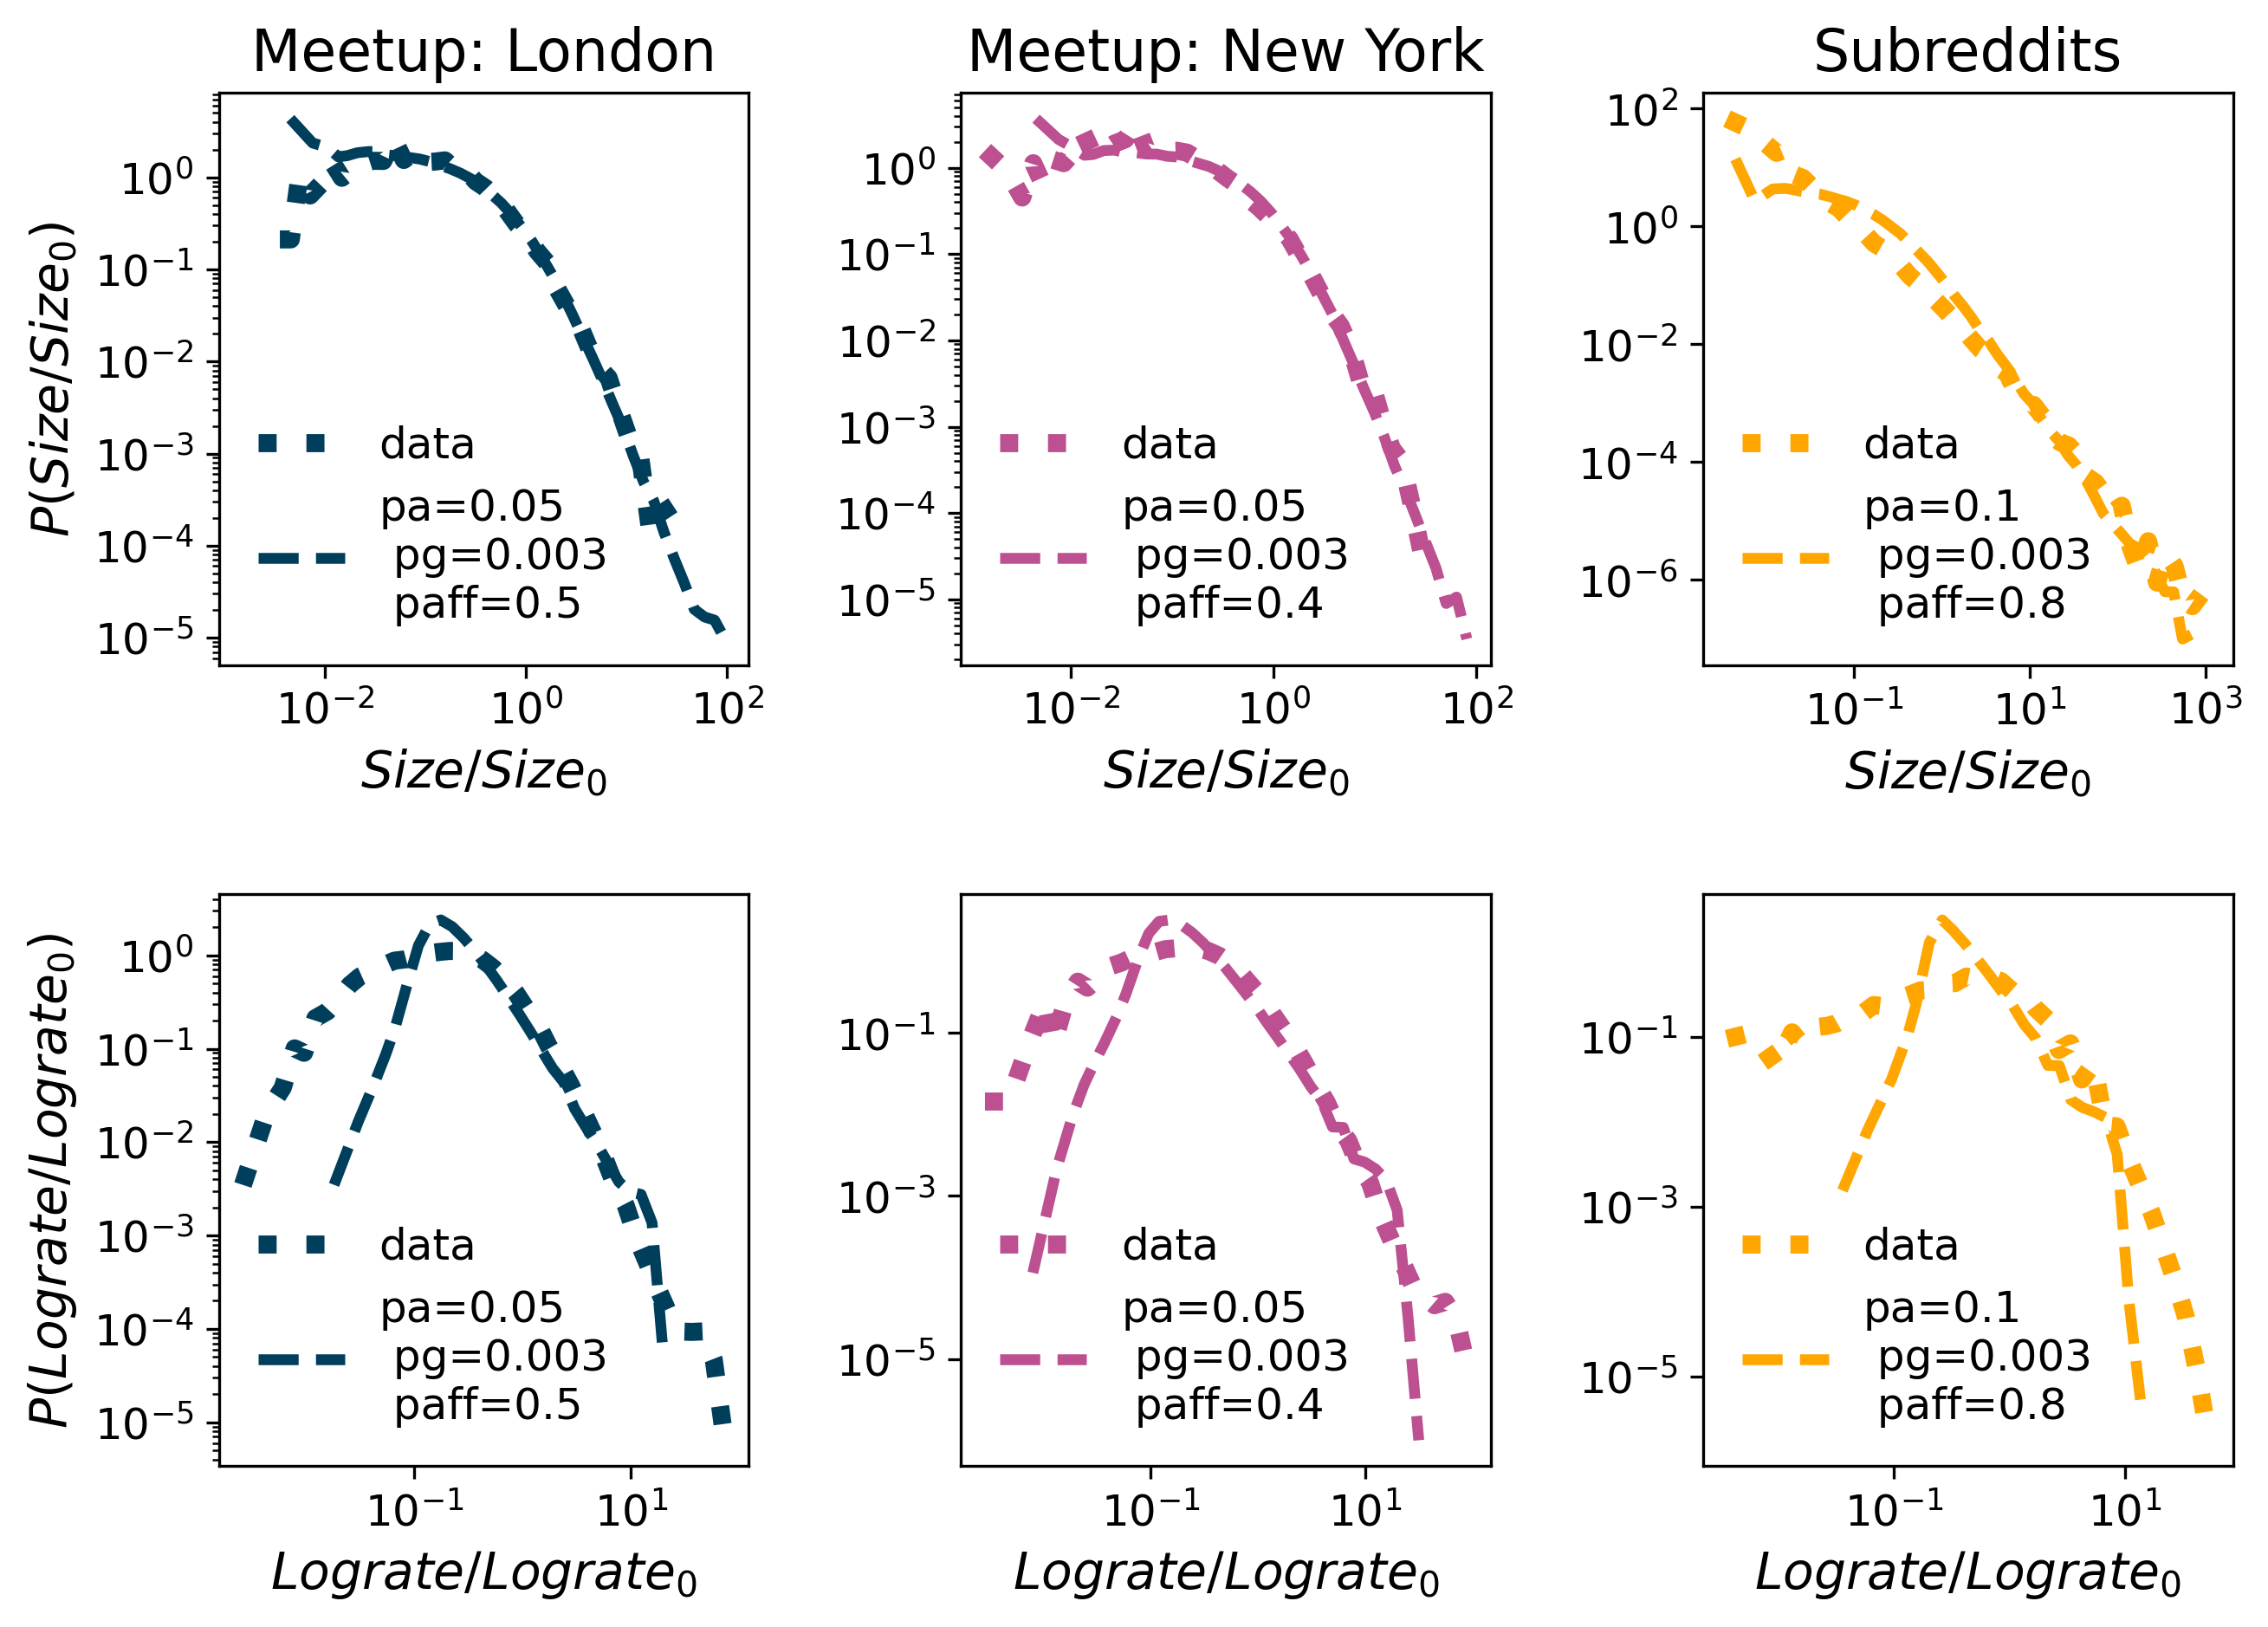
\includegraphics[width=0.8\linewidth]{Figures/figures/Fig4.png}
	\caption{The comparison between empirical and simulation distribution for group sizes (top panel) and logrates (bottom panel).}
	\label{fig:fig6}
\end{figure}


%\section{Discussion and conclusions \label{sec:con}}

%The growth of the cities and companies has attracted the attention of researchers in the previous few decades \cite{fazio2015pareto, amaral1997scaling,}. It is not surprising if we keep in mind that their growth determines other processes essential for the functioning of cities and economies. In the cities, economic and innovation growth scale with their size \cite{bettencourt2007growth}. The understanding of growth and segmentation of economic systems are essential for the long-term prediction of their evolution, and risk assessment \cite{}. The growth of social groups and social system segmentation has been slightly overlooked since the focus was mainly on the structure of social networks and their evolution.
%However, several works have studied the growth of social groups and tried to provide some insights into mechanisms that drive the growth and segmentation of social systems \cite{}.  

%The results of our empirical analysis and theoretical modeling show that there are universal growth rules that govern the growth of social groups in these systems. Through rigorous empirical analysis of the growth of social groups in three systems, Meetup groups located in London and New York, and Reddit, we show that the distribution of group sizes in these systems has log-normal normal behavior. The empirical distributions of normalized sizes of the groups created in different years fall on top of each other and have the same values of parameters for the same system. Furthermore, the distributions for Meetup groups located in London and New York have similar model parameter values, suggesting that groups' growth in these two systems are similar. Numerical simulations further confirm these findings. By tuning our model's parameters, we can reproduce the distribution of group sizes in all three systems.  

%Our results show that while the processes that govern the growth of social groups in studied social systems are the same, their importance varies among systems. The analysed groups grow through two mechanisms \cite{zheleva2009co}: members join a group that is chosen according to their interests or social relations with the group's members.
%%The analysed groups grow through two mechanisms \cite{zheleva2009co}: members join a group that is chosen either according to their interests or according to their social relations with members of the group.


%The number of members in the system is growing, as well as the number of groups. The empirical distribution of growth rates differs for Meetup and Reddit. The observed differences can be explained by different modalities of interactions between their members. Meetup members need to invest more time and resources to interact with their peers. The events are localised in time and space, and thus the influence of peers in selecting another social group may be limited. On the other hand, Reddit members do not have these limitations. The interactions are online, asynchronous, and thus not limited in time. The influence of peers in choosing new subreddits and topics thus becomes more important. The inspection of numerical simulations confirms these observations. The values of $p_{aff}$ parameters for Meetup and Reddit imply that social connections in diffusion between groups are more critical in Reddit than in Meetup.   

%Gibrat's law is the first empirical law used by researchers to describe and explain the growth and segmentation of various socio-economical systems, including cities and firms. The possibility of application of common law to the growth of social groups in different systems indicates the existence of universal growth patterns and mechanisms that govern that growth \cite{}. Detailed and rigorous empirical analysis of the growth of the cities and firms showed that it goes beyond Gibrat's law \cite{}. Our and the work of other researchers \cite{zheleva2009co} confirm that these findings also hold for the growth of social groups. The analysis of monthly growth rates shows that these rates are log-normally distributed and depend on the size of a group. Furthermore, we cannot reduce the model proposed in this work to the law of proportional growth. Although our analysis shows that Gibrat's law does not apply to the growth of social groups, our findings confirm that universal patterns characterise this growth. 

%The results presented in this paper contribute to our knowledge of the growth and segmentation of socio-economical systems. Our rigorous analysis shows that the distribution of sizes of groups for studied systems follows a log-normal distribution. The findings of the previous research suggested the power-law behavior of this distribution. A detailed and comprehensive analysis of distributions of group sizes in social systems is needed. These and future results will help us better understand the growth and segmentation of social systems and predict their evolution and sustainability. 
%----------------------------------------------------------------------------------------

\section{Distributions fit}

%We compute the log-likelihood ratio $R$, and $p$-value between different distributions and log-normal fit \cite{clauset2009power} to determine the best fit for the group size distributions. Distribution with a higher likelihood is a better fit. The log-likelihood ratio R then has a positive or negative value, indicating which distribution represents a better fit. To choose between two distributions, we need to calculate p-value,  to be sure that R is sufficiently positive or negative and that it is not the result of chance fluctuation from the result that is close to zero. If the p-value is small, $p<0.1$, it is unlikely that the sign of R is the chance of fluctuations, and it is an accurate indicator of which model fits better. \\

%Table \ref{tab:fit-data} summarizes the findings for empirical data on group size distributions from Meetup groups in London, Meetup groups in New York and Reddit. Using the maximum likelihood method, we obtain the parameters of the distributions \cite{powerlaw}. The results indicate that log-normal distribution is the best fit for all three systems.  Figure \ref{fig:fitdata} shows the distributions of empirical data as well as log-normal fit on data. For Meetup data, we present fit on stretched exponential distribution, which very well fits a large portion of data. For subreddits, distribution is broad and, potentially, resembles power-law. Still, log-normal distribution is a more suitable fit.

\begin{table}[!h]
	\centering
	\caption{The likelihood ratio R and p-value between different candidates and \textbf{lognormal} distribution for fitting the distribution of \textbf{groups sizes} of Meetup groups in London, New York and in Reddit. According to these statistics, the lognormal distribution represents the best fit for all communities. \\ }
	\begin{tabular}{|c||cc||cc||cc|}
		\hline
		\multirow{2}{*}{\begin{tabular}[c]{@{}c@{}}distribution \end{tabular}} & \multicolumn{2}{c||}{\begin{tabular}[c]{@{}c@{}}Meetup\\ city London\end{tabular}} & \multicolumn{2}{c||}{\begin{tabular}[c]{@{}c@{}}Meetup\\ city NY\end{tabular}} & \multicolumn{2}{c|}{Reddit}                    \\ \cline{2-7} 
		& \multicolumn{1}{c|}{R}                             & p                            & \multicolumn{1}{c|}{R}                           & p                          & \multicolumn{1}{c|}{R}         & p             \\ \hline \hline \hline
		exponential                                                                            & \multicolumn{1}{c|}{-8.64e2
			%-864.86
		}                       & 8.11e-32                     & \multicolumn{1}{c|}{-8.22e2}                     & 6.63e-26                   & \multicolumn{1}{c|}{-3.85e4} & 1.54e-100     \\ \hline
		\begin{tabular}[c]{@{}c@{}}stretched \\ exponential\end{tabular}                       & \multicolumn{1}{c|}{-3.01e2}                       & 1.00e-30                      & \multicolumn{1}{c|}{-1.47e2}                     & 7.78e-8                    & \multicolumn{1}{c|}{-7.97e1}    & 5.94e-30      \\ \hline
		power law                                                                              & \multicolumn{1}{c|}{-4.88e3}                      & 0.00                         & \multicolumn{1}{c|}{-4.57e3}                    & 0.00                       & \multicolumn{1}{c|}{-9.39e2}   & 4.48e-149 \\ \hline
		\begin{tabular}[c]{@{}c@{}}truncated \\ power law\end{tabular}                         & \multicolumn{1}{c|}{-2.39e3}                      & 0.00                         & \multicolumn{1}{c|}{-2.09e3}                    & 0.00                       & \multicolumn{1}{c|}{-5.51e2}   & 2.42e-56      \\ \hline
	\end{tabular}
	\label{tab:fit-data}
\end{table}

\begin{figure}[!h]
	\centering
	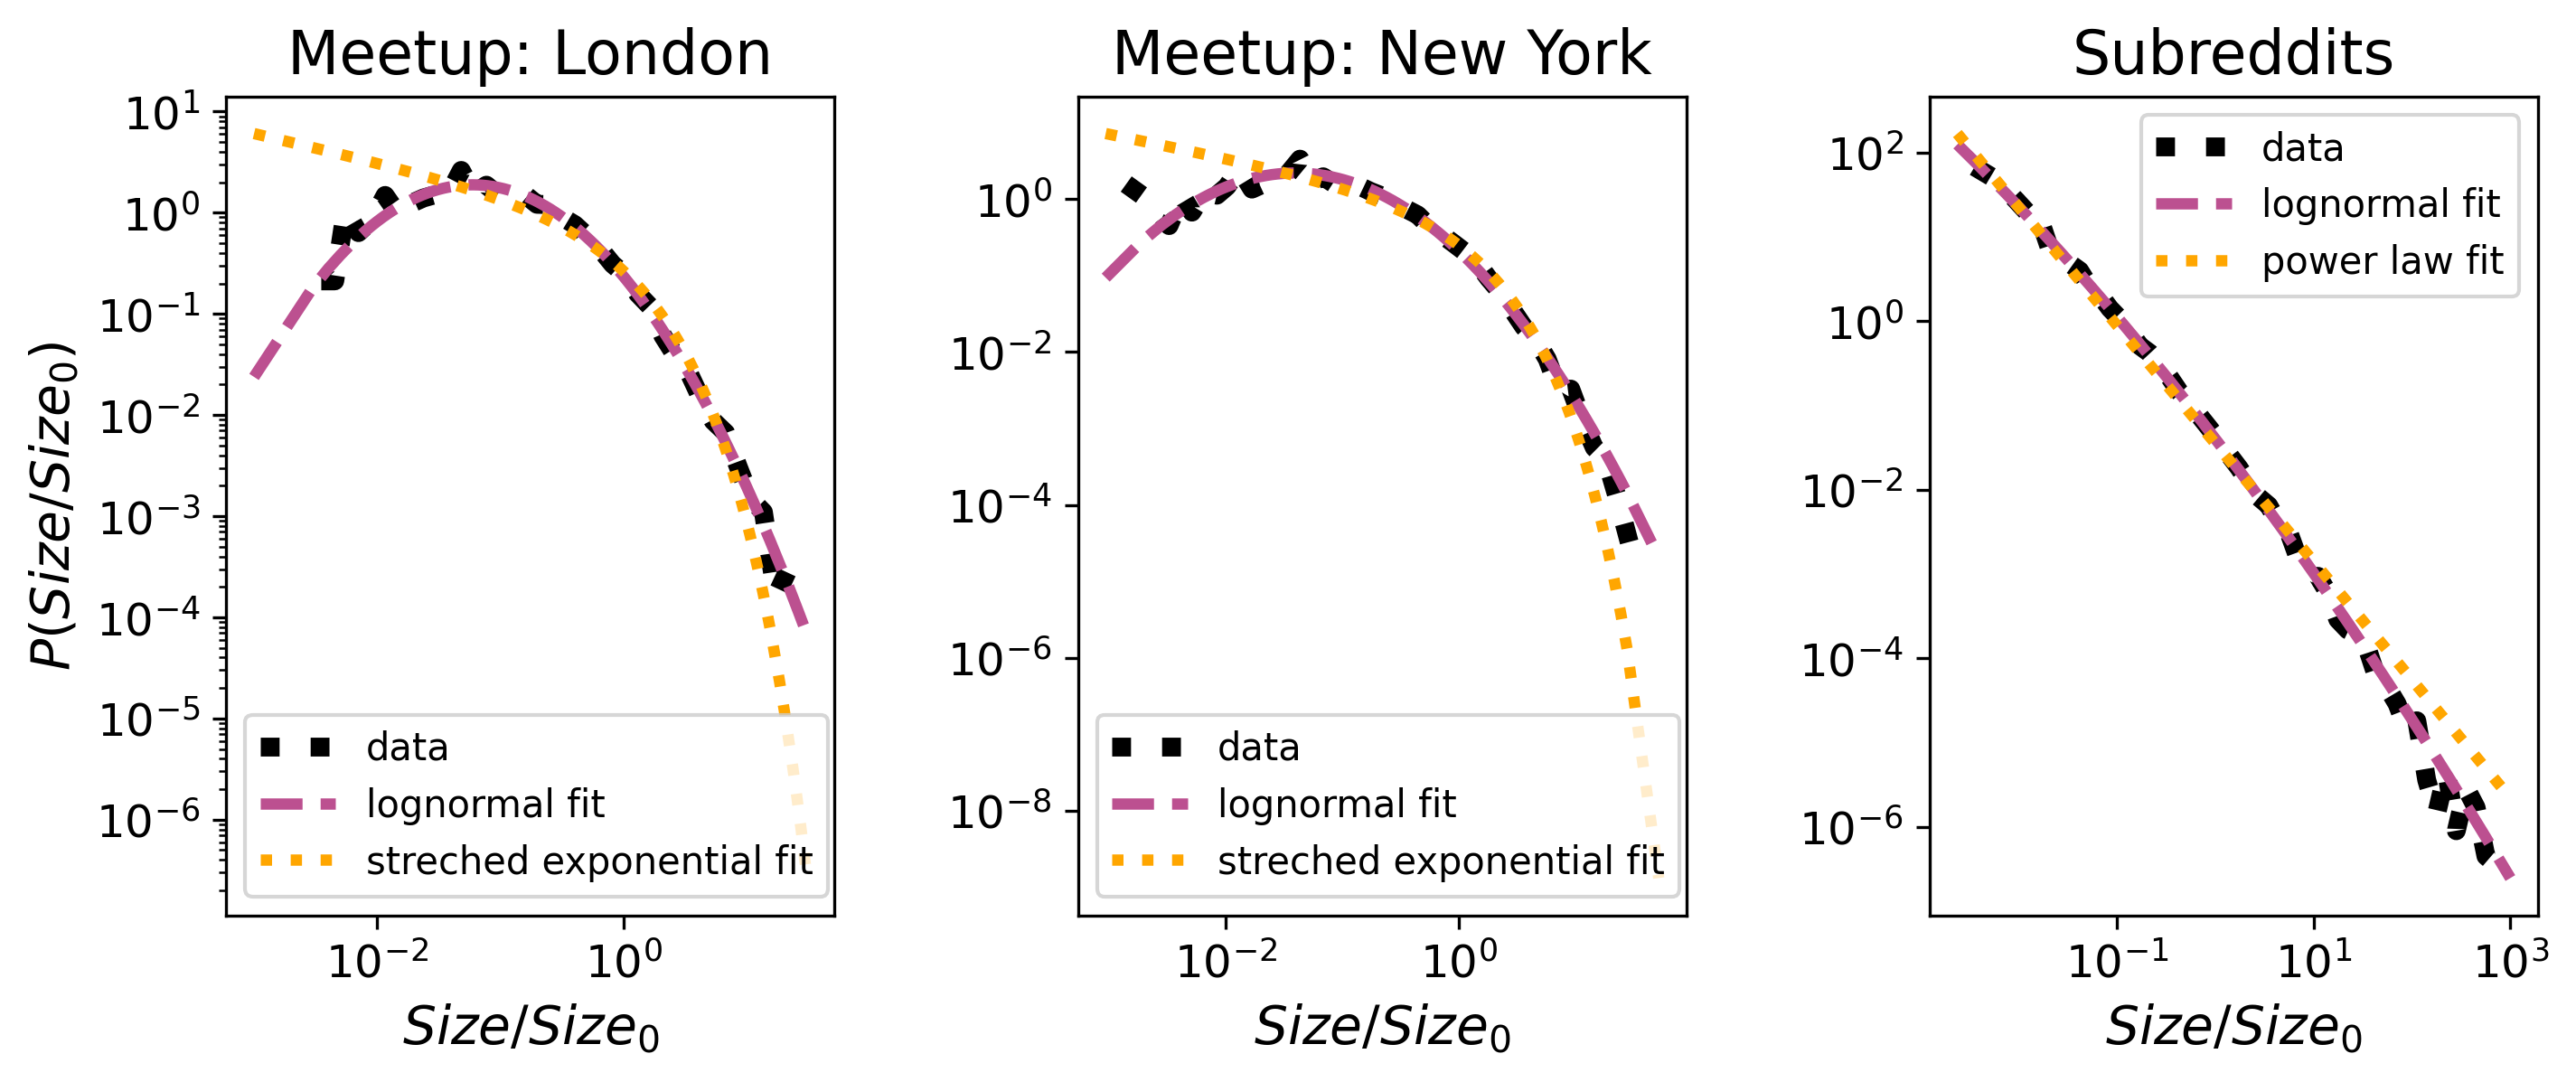
\includegraphics[width=0.9\linewidth]{figures/FigA1_data.png}
	\caption{The comparison between log-normal and stretched exponential fit to London and NY data,  and between log-normal and power law for Subreddits. The parameters for log-normal fits are 1) for city London $\mu=-0.93$ and $\sigma = 1.38$, 2) for city NY $\mu=-0.99$ and $\sigma = 1.49$, 3) for Subreddits $\mu=-5.41$ and $\sigma = 3.07$.  }
	\label{fig:fitdata}
\end{figure}

%We use the same methods to estimate the fit for simulated group size distributions on Meetup groups in London, New York, and Subreddits. Table \ref{tab:fit_model} shows the results of the log-likelihood ratio R and $p$-value between different distributions. We conclude that log-normal distribution is most suitable for simulated group size distributions. Plotting log-normal and stretched exponential fit on data, Fig. \ref{fig:fit_model} we confirm our observations.  
% Please add the following required packages to your document preamble:
% \usepackage{multirow}
\begin{table}[h]
	\centering
	\caption{The likelihood ratio R and p-value between different candidates and \textbf{lognormal}
		distribution for fitting the distribution of \textbf{simulated group sizes} of Meetup groups in London, New York and Reddit. According to these statistics, the lognormal distribution
		represents the best fit for all communities. \\}
	\begin{tabular}{|c||cc||cc||cc|}
		\hline
		\multirow{2}{*}{\begin{tabular}[c]{@{}c@{}}distribution \end{tabular}} & \multicolumn{2}{c||}{\begin{tabular}[c]{@{}c@{}}Meetup\\ city London\end{tabular}} & \multicolumn{2}{c||}{\begin{tabular}[c]{@{}c@{}}Meetup\\ city NY\end{tabular}} & \multicolumn{2}{c|}{Reddit}                \\ \cline{2-7} 
		& \multicolumn{1}{c|}{R}                              & p                           & \multicolumn{1}{c|}{R}                            & p                         & \multicolumn{1}{c|}{R}         & p         \\ \hline \hline \hline
		exponential                                                                            & \multicolumn{1}{c|}{-6.27e4}                      & 0.00                        & \multicolumn{1}{c|}{-5.11e4}                    & 0.00                      & \multicolumn{1}{c|}{-1.26e5} & 7.31e-125 \\ \hline
		\begin{tabular}[c]{@{}c@{}}stretched\\ exponential\end{tabular}                        & \multicolumn{1}{c|}{-1.01e4}                      & 1.96e-287                    & \multicolumn{1}{c|}{-6.69e3}                     & 1.46e-93                  & \multicolumn{1}{c|}{-1.39e4} & 0.00      \\ \hline
		power law                                                                              & \multicolumn{1}{c|}{-2.29e5}                     & 0.00                        & \multicolumn{1}{c|}{-3.73e5}                   & 0.00                      & \multicolumn{1}{c|}{-4.38e4} & 0.00      \\ \hline
		\begin{tabular}[c]{@{}c@{}}truncated\\ power law\end{tabular}                          & \multicolumn{1}{c|}{-9.28e4}                      & 0.00                        & \multicolumn{1}{c|}{-1.55e5}                   & 0.00                      & \multicolumn{1}{c|}{-9.12e4} & 0.00      \\ \hline
	\end{tabular}
	\label{tab:fit_model}
\end{table}


\begin{figure}[h]
	\centering
	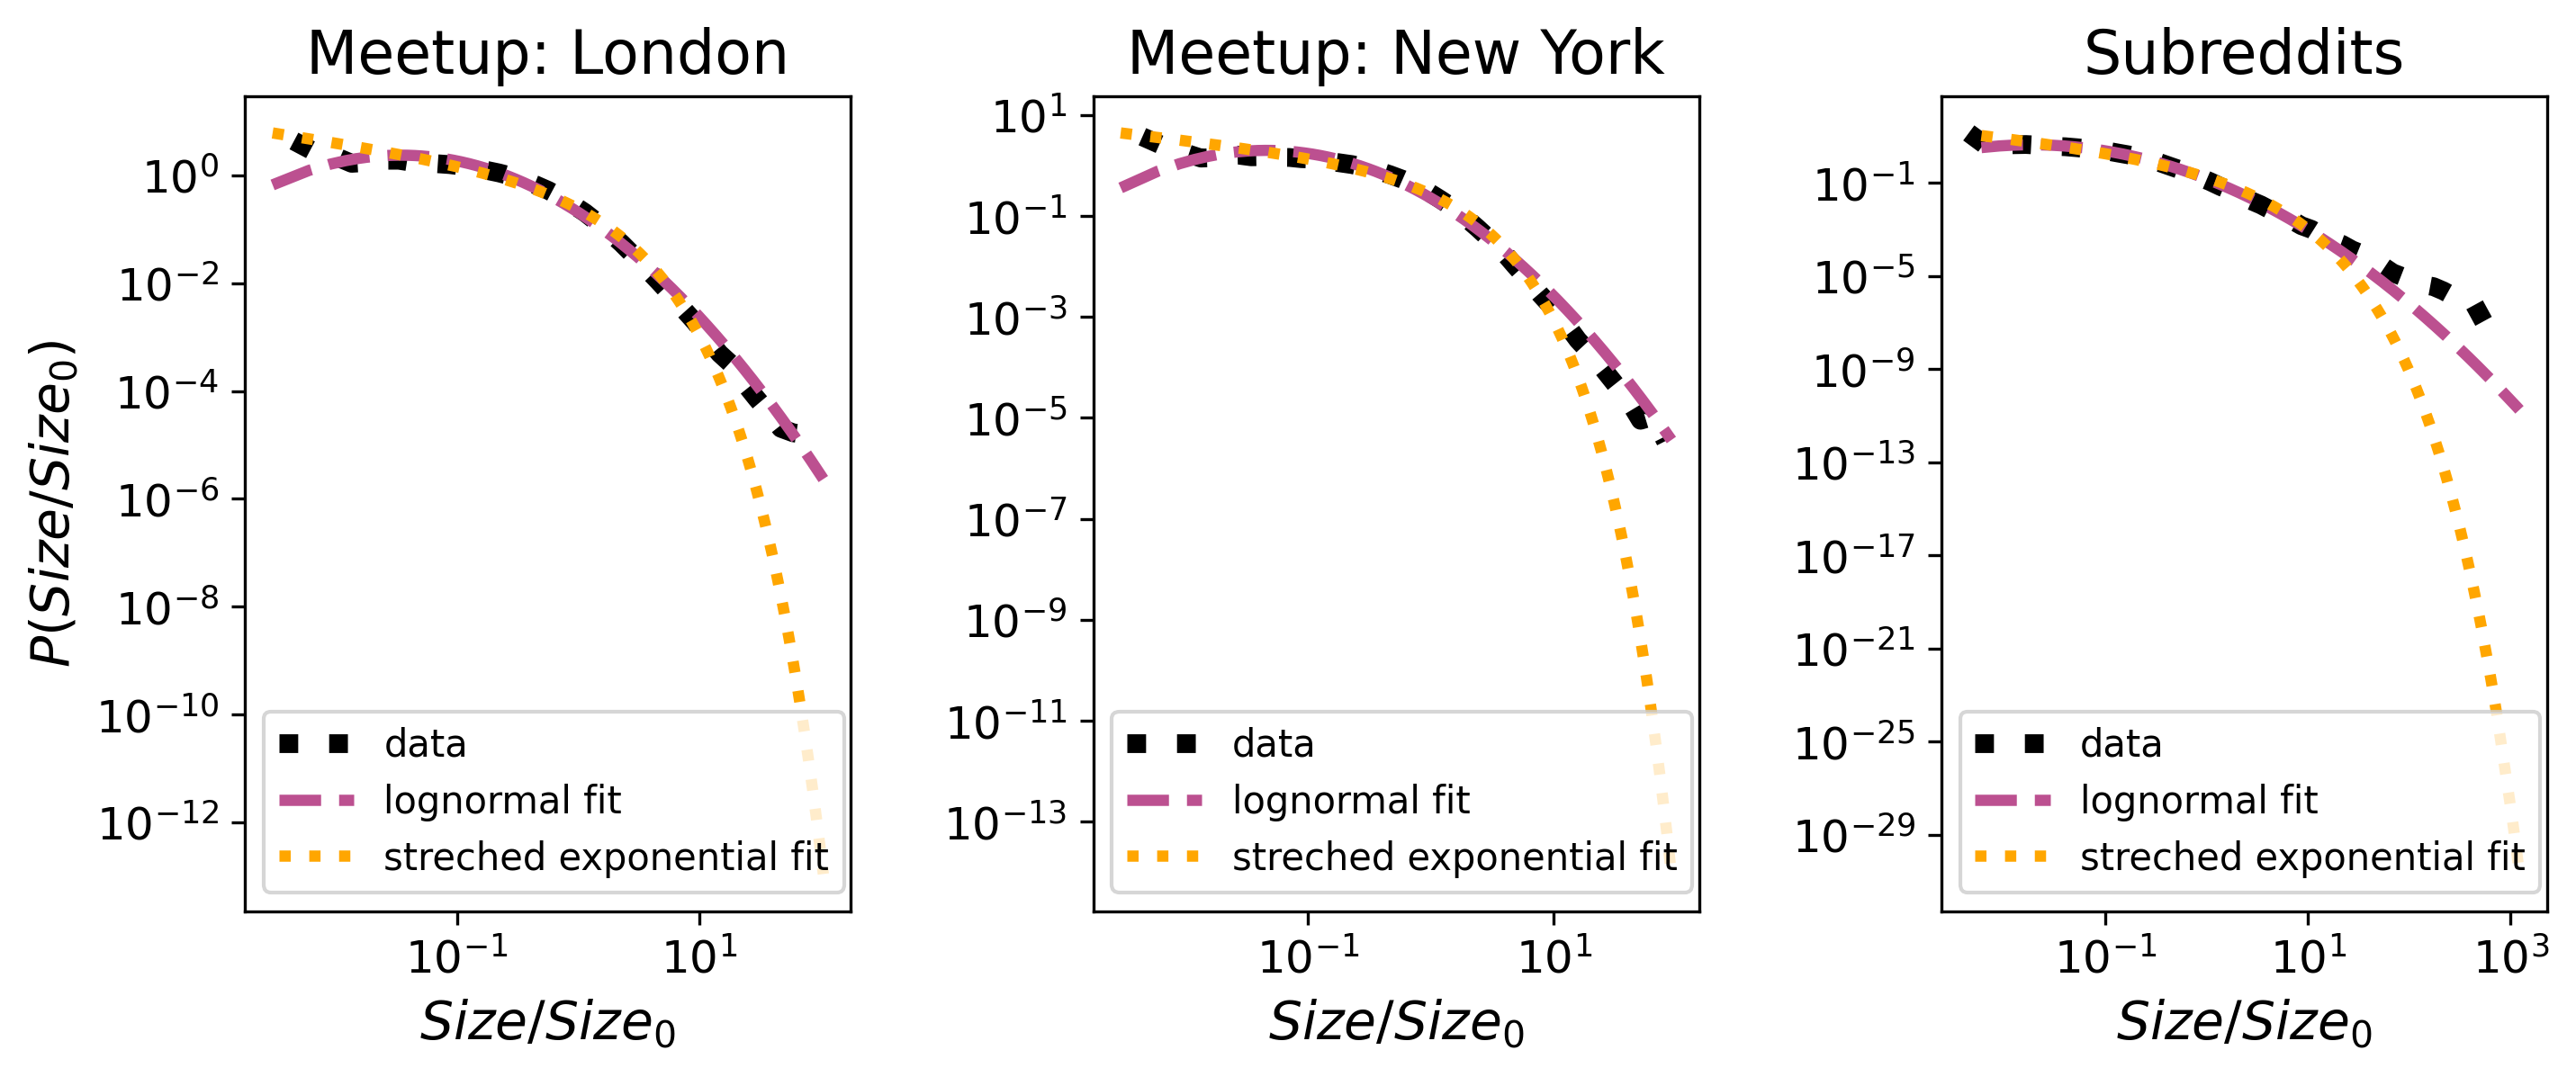
\includegraphics[width=0.9\linewidth]{figures/FigA2-model.png}
	\caption{The comparison between lognormal and stretched exponential fit to simulated group sizes distributions. The parameters for log-normal fits are 1) for city London $\mu=-0.97$ and $\sigma = 1.43$ , 2) for city NY $\mu=-0.84$ and $\sigma = 1.38$ , 3) for Subreddits $\mu=-1.63$ and $\sigma = 1.53$. }
	\label{fig:fit_model}
\end{figure}


%\section{The model for social groups growth}
%In the groups growth model, at each step, new users join the network, while old users are active with probability $p_a$. Active users can create new group with probability $p_g$. Otherwise, with probability $p_{aff}$, they perform diffusion linking. With probability, $1-p_{aff}$ users join a random group. Figure \ref{fig:model_comp}, top row, shows that group sizes distributions follow log-normal distribution. The affiliation parameter $p_{aff}$ influences the width of distributions, so for larger $p_{aff}$, we find larger groups in the network.   If, instead of random linking, users with probability  $1-p_{aff}$, choose to join to larger groups, group sizes distribution change significantly. Similar to affiliation model \cite{zheleva2009co}, group sizes have power-law distribution, see bottom row on Figure \ref{fig:model_comp}.




